\label{ch:research_premises}
\section{Research Objectives}
After the description of the experimental apparatuses that we used, and a basic explanation of the main principles in glass polishing, we can present the main ideas and goals of the project.
\\
Due to the grinding and polishing process in optics manufacturing, contaminants can leak into the surface of the glass from both the water and the polishing suspension, possibly causing issues in the optical property of the final product.
\\
Our primary research objectives were:
\begin{enumerate}
    \item To confirm the presence of contaminants and to definitively confirm whether contamination actually occurs.
    \item To quantify the magnitude of this effect by measuring the concentration of contaminants at the surface.
    \item To investigate whether the process parameters, like polishing time or polish concentration, can have an influence on the result.
\end{enumerate}
A crucial part of our experience was to investigate whether all these evaluations could be done using a LIBS apparatus.

\section{Polishing Parameters}
\label{sec:pol_parameter}
After having thought about the parameters we could vary, we settled on a collection of variables that we identified as the most relevant:
\begin{itemize}
    \item Polishing time: by increasing the contact time we expect to see changes in the amount of concentration found at the surface.
    \item Polishing agent: expecting that the physical and chemical properties of different agents could have a different interaction with the glass. The two main polishing agents used in optics manufacturing are aluminum oxide (\ce{Al2O3}) and cerium oxide (\ce{CeO2}). The latter also usually contains traces of other elements like carbon or lanthanum.
    \item Type of water: tap water could impact the process by introducing new contaminants. Also, tap and distilled water can differ for chemical properties too, the pH of tap water is usually around 7.4 and distilled water is slightly more acidic with a pH of 5.7, due to the presence of a small amount of carbon dioxide that gets instantly dissolved into the water from the atmosphere [ph water paper].
    \item Polish concentration: the common concentrations used in optic manufacturing are between 5\% to 30\% in mass, where the percentage indicates the fraction of the mass of the polishing agent relative to the total weight of the slurry. Concentration influences both the mechanical properties of the solution, by physically having more particles interacting with the surface, and the chemical ones, by changing the alkalinity.
    \item Type of glass: glasses with different compositions are used in optics because their refractive index is strongly dependent on the density of the material and by introducing different and heavier elements in the glass, the manufacturer can tune its optical properties to the desired ones. Having a high concentration of different elemental species inside the glass could change the parameters that regulate diffusion at the surface.
\end{itemize}

\section{Theoretical Prediction}
\label{sec:theoretical_prediction}
As already mentioned in Chapter~\ref{sec:grinding_glass}, the description of the chemical-mechanical polishing is extremely complex, and it would be difficult to develop a model to predict and fit the results to the LIBS measurement.
\\
The simplest approach to describe the presence of contaminants in the glass is diffusion. Specifically, “normal” diffusion, where the concentration follows the two Fick’s laws. In particular, a solution for the second Fick’s law states:
\begin{align}
    C\left(x,t\right)=C_0\operatorname{erfc}\left(\frac{x}{2\sqrt{Dt}}\right) \label{eq:second_fick}
\end{align}
In the case of our LIBS measurements, we are not measuring depth resolved data. The laser ablates all the material in a small portion of the surface, and we measure the concentration of all the species that are present from the surface level to the deepest part of the ablated region. We are therefore measuring a quantity that is proportional to the integral of the concentration.
\\
Is it possible to obtain the analytical solution of the integral of the error function, by looking at some tables we find that:
\begin{align}
    \int\operatorname{erfc}\left(az\right)dz=z\operatorname{erfc}\left(az\right)-\frac{1}{a\sqrt\pi}\exp{\left(-a^2z^2\right)} \label{eq:integral_erfc}
\end{align}
In our case the parameter $a$ is equal to $\frac{1}{2\sqrt{Dt}}$. The integral is then evaluated over an interval that starts at 0, that we take as the surface level, and ends at a distance $d_a$, which is the maximum depth of the ablation. It also makes sense to normalize the expression relative to the length by dividing the integral by $d_a$.
\\
The final expression is therefore: 
 \begin{align}
    \overline{C}\left(d_{a},t\right)=\frac{C_{0}}{d_a}\int_{0}^{d_{a}}\operatorname{erfc}\left(\frac{x}{2\sqrt{Dt}}\right)\operatorname{d}x=C_{0}\left[d_{a}\operatorname{erfc}\left(\frac{d_{a}}{2\sqrt{Dt}}\right)-2\sqrt{\frac{Dt}{\pi}}\left[\exp\left(-\frac{d_{a}^{2}}{4Dt}\right)-1\right]\right]\frac{1}{d_a} \label{eq:c_bar_equation}
 \end{align}
There are two functional contributions to the expression:
\begin{align}
    g(t) &= d_{a\ }\operatorname{erfc}\left(\frac{d_a}{2\sqrt{Dt}}\right) \label{eq:g_t} \\
    \\[1pt]
    h(t) &= 2\sqrt{\frac{Dt}{\pi}}\left[\exp{\left(-\frac{d_a^2}{4Dt}\right)}-1\right] \label{eq:h_t}
\end{align}
In this way $\overline{C}$ can be written as $\overline{C} = g(t) + h(t)$
\\
By plotting the two contributions and the total function in a logarithmic plot, we can see that $g(t)$ and $h(t)$ intersect.
\\
The time value at the intersection point, $t_s$, separates the domain in two regions:
\begin{figure}[H]
   \centering
   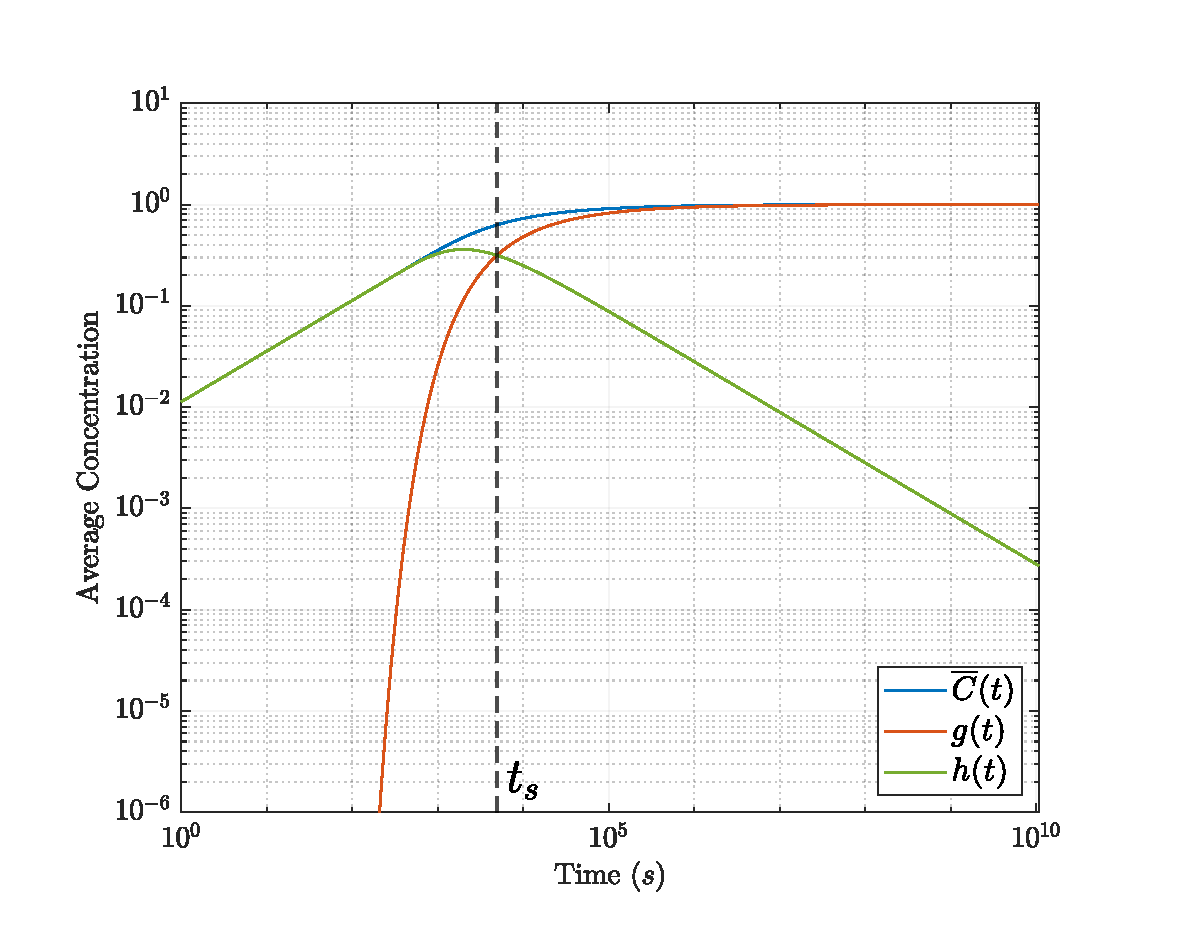
\includegraphics[width = \textwidth]{chapter_3/theoretical_cons/conc3Functions.pdf} 
   \caption{The average concentration and the two functional components. }
   \label{fig:c_bar_plot}
\end{figure}
For $t<t_s$, $h(t)$ is the dominant contribution, and the overall function behaves linearly.
\\
For $t>t_s$, $g(t)$ becomes the dominant contribution. Since $g(t)$ tends to $C_0$, $\overline{C}$ will also tend to the same parameter. Physically, this behavior represents the time values for which the saturation condition, with a homogeneous concentration equal to $C_0$, has been reached in the spatial region between 0 and $d_a$. 
\\
Considering that $D$ is always multiplying $t$, a change in the value of the diffusion coefficient, translates in a rigid shift to the left, by a value equal to $\log_{10}(D)$, of the whole function.
\\
Therefore, looking at a fixed interval of time between $t_1$ and $t_2$, two cases can be distinguished:
\\
If $t_s >> t_2$, corresponding to small values of $D$, the behavior is linear inside the considered region, and saturation is not reached.
\begin{figure}[H]
   \centering
   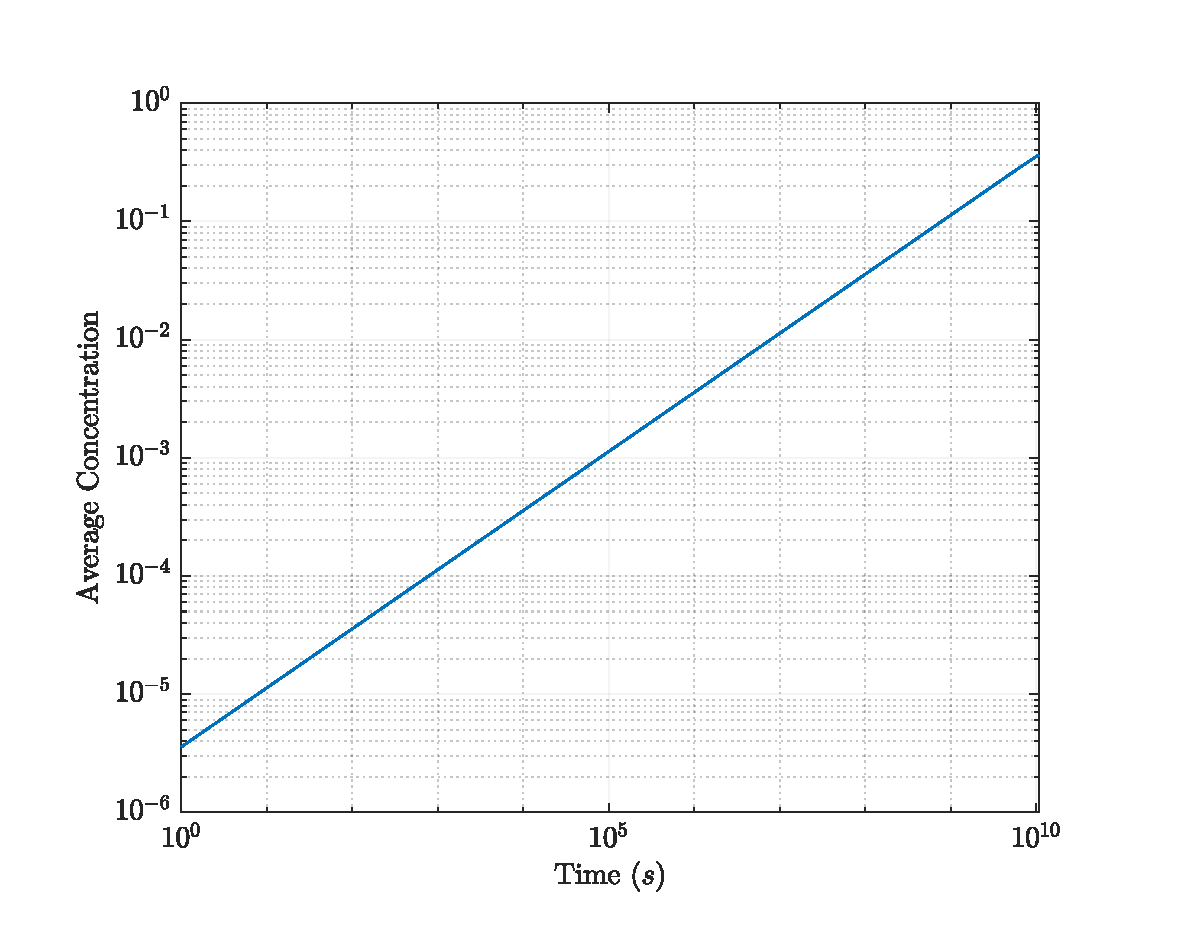
\includegraphics[width = \textwidth]{chapter_3/theoretical_cons/concRegim_linear.pdf} 
    \vspace*{-30pt}
   \caption{Linear behavior of $\bar{C}$ for $\protect t_s >> t_2$.}
   \label{fig:c_bar_linear}
\end{figure}
If $t_s ~ t_1$, corresponding to the case of a high value of $D$, saturation is reached almost instantly, and the behavior cannot be considered linear anymore.
\begin{figure}[H]
   \centering
   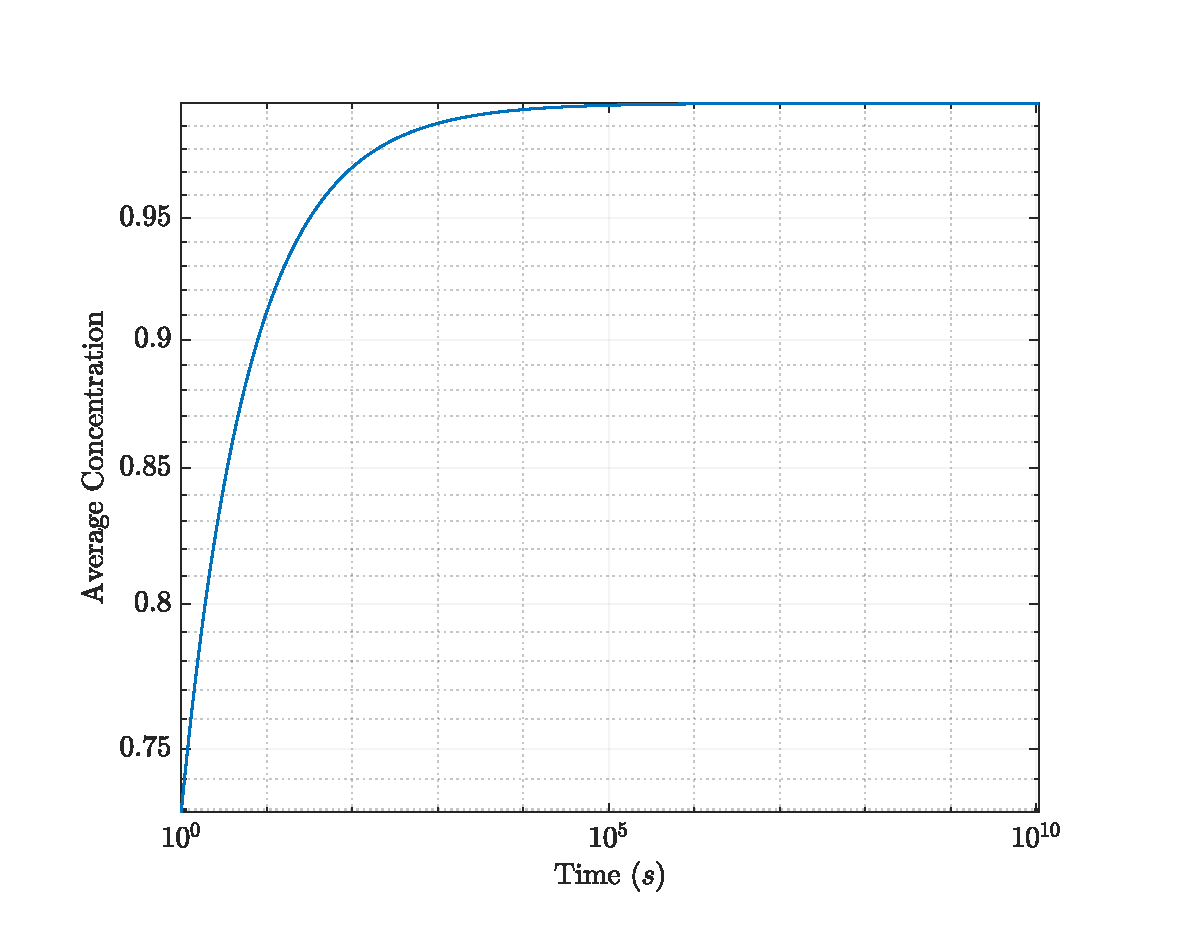
\includegraphics[width = \textwidth]{chapter_3/theoretical_cons/concRegim_exp.pdf} 
    \vspace*{-30pt}
   \caption{Non-linear behavior of $\bar{C}$ for $\protect t_s ~ t_1$.}
   \label{fig:c_bar_non_linear}
\end{figure}
If $t_s \in [t_1, t_2]$, both behaviors are present, and saturation is reached after a period of linear regime.
\begin{figure}[H]
    \centering
    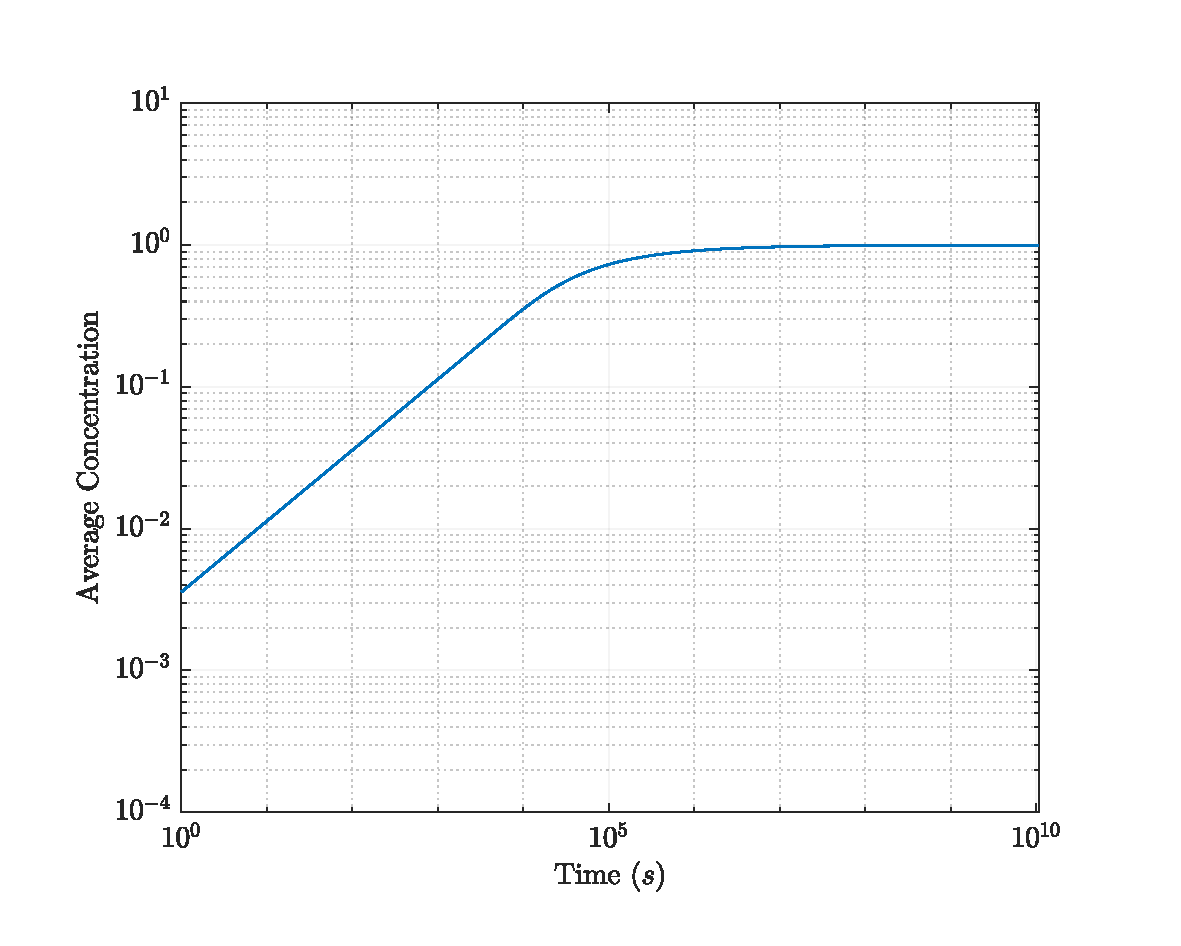
\includegraphics[width = \textwidth]{chapter_3/theoretical_cons/concRegim_mixed.pdf} 
     \vspace*{-30pt}
    \caption{General behavior of $\bar{C}$ for  $t_s \in [t_1, t_2]$.}
    \label{fig:c_bar_mixed}
 \end{figure}
This discussion is relevant because, if the predominant physical mechanism causing the presence of contaminants in the glass is actually diffusion, we should be able to estimate the value of the diffusion constant by comparing $\bar{C}$ to the data found with LIBS measurements.

\chapter{Experimental Setup}
\label{ch:experimental_setup}


\section{LIBS}
\label{sec:LIBS_apparatus}

\subsection{Description of the apparatus}
\label{sec:Description_of_the_apparatus}

As already anticipated in Chapter~\ref{sec:LIBS}, LIBS setup components are multiple.
\\
This analysis technique needs active elements capable of providing the optical energy needed for plasma formation, and a collection of optical and electronic elements capable of collecting and analyzing emitted light from the plasma.
\\
Due to the large field of application of this technique [Source of the different applications], LIBS setups are expected to vary both in size (static vs portable) and complexity.
\\
Generally, LIBS setups all share the same main elements that are listed below:
\begin{enumerate}
    \item The laser source.
    \item The optical system that focuses the laser light on the sample surface.
    \item A target holder.
    \item The light collection system, needed to convey the generated radiation to the detector.
    \item The detection system, capable of spectrally dispersing the collected light and measuring it using a digital sensor.
    \item A computer to control each previously cited element and to create the final spectrum.
\end{enumerate}
The LIBS measurements presented in this thesis have all been carried out using the same apparatus, a custom-made version of the CORALIS system by Lasertechnik Berlin with the following characteristics.

\subsubsection{Laser Source}
\label{subsubsec:laster_source}
A solid state, Nd:YAG laser source has been employed in this setup. The system gave us the possibility of tuning the laser pulse energy from less than $1 \: mJ$,  to more than 100.
\\
The Nd:YAG laser was operated at its fundamental wavelength of $1064 \: nm$ and in the Q-Switching regime, in order to achieve the high enough pulse power capable of igniting the plasma. This pulsed laser regime gives a typical duration of each pulse in the order of $5-10\: ns$ [Handbook of LIBS (other sources are possible)] and in the case of the CORALIS system the machine can provide up to 20 pulses per second, with a repetition rate of 20 Hz.

\subsubsection{Spectrometer}
\label{subsubsec:spectrometer}
The choice of the spectrometer is also dependent on the type of application and can range from the use of very simple and inexpensive components, such as line filters capable of monitoring a single predetermined wavelength, to sophisticated spectrographs allowing for the simultaneous analysis of a large spectral region.
\\
The commercially available CORALIS has only one echelle spectrometer that operates in the near-UV range (from 190 to $430 \: nm$) and has a spectral resolution that spans from 13 to $35 \: pm$, with a sensitivity of [].
\\
The modified model that we employed has an additional spectrometer that operates in the visible range (from 405 to $802\: nm$) with a spectral resolution of around $4 \: pm$, with a sensitivity of [].
[we are not sure on the value of the resolution of the Visible spectrometer, and we do not have yet the values for the sensitivity]
\\
The overall spectral region that we could analyze was therefore from 200 to $800 \: nm$.

\subsection{Parameters Chosen}
\label{subsec:parameters_chosen}
The choice of the LIBS parameters is a very crucial step in the analysis process since the quality of the results obtained from the measurements is strongly dependent on their values. In general, there are no parameters that are universally optimal, and their value changes based on the type of material, the geometry of the surface, and the element species that are being investigated.
\\
In order to arrive at the final values we employed, a thorough experimental process has been carried out.
\\
The parameters on which we had full choice were the sequent:
\begin{enumerate}
    \item Laser pulse energy.
    \item Gate width.
    \item Delay time.
    \item Detector gain.
    \item Spatial distribution of the measured points on the sample surface.
    \item Number of points per measurement.
    \item Number of laser pulses per measurement.
    \item Number of cleaning pulses before the measurement.
\end{enumerate}
The choice process for the parameters started by analyzing an NZK-7 glass sample from Schott [need the citation]. The glass sample did not undergo any post-processing phase, like grinding or polishing. From now on we will refer to this type of sample as “RAW”.
\\
The first parameter on which we focused our attention was the laser pulse energy. 
\subsubsection{Pulse Energy}
\label{subsubsec:pulse_energy}
Silica glass absorbs radiation very inefficiently in the frequency range of the laser of the apparatus we used, as it is clear from Figure~\ref{fig:glass_transmittance} at $1064 \: nm$ the glass transmittance is basically 100\%. 
\begin{figure}[H]
    \centering
    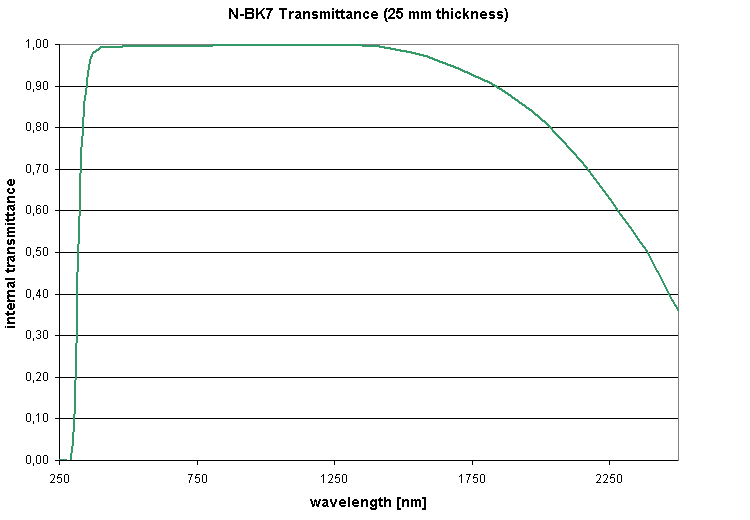
\includegraphics[width = 0.7\textwidth]{chapter_3/tests_graphs/glass_transmittance.png} 
    \caption{Transmittance of N-BK7 glass.}
    \label{fig:glass_transmittance}
 \end{figure}
 Also, in general, the lack of surface features due to polishing and grinding reduces even more the possibility of absorption. To achieve the conditions for breakdown at the surface, a high laser pulse energy must be utilized.
 \\
Tests were carried out from a lower value of $6 \:mJ$ to a higher value of $15\: mJ$.
\\
In Figure~\ref{fig:test_NZK7_6mj} and Figure~\ref{fig:test_NZK7_6mj_zoom} we can see that we already have a good spectrum even with just $6 mJ$.
\begin{figure}[H]
    \centering
    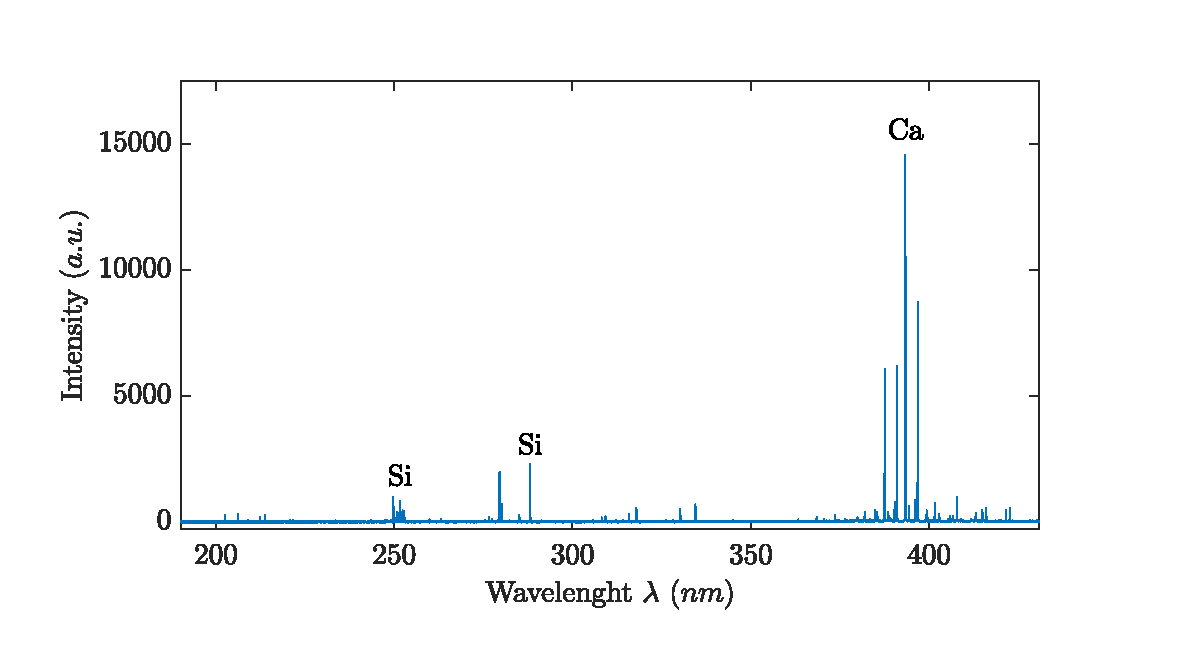
\includegraphics[width = \textwidth]{chapter_3/tests_graphs/test_NZK7_6mj.pdf} 
     \vspace*{-30pt}
    \caption{$\protect 6 \: mJ$ - Spectrum of NZK-7 glass.}
    \label{fig:test_NZK7_6mj}
\end{figure}
\begin{figure}[H]
    \centering
    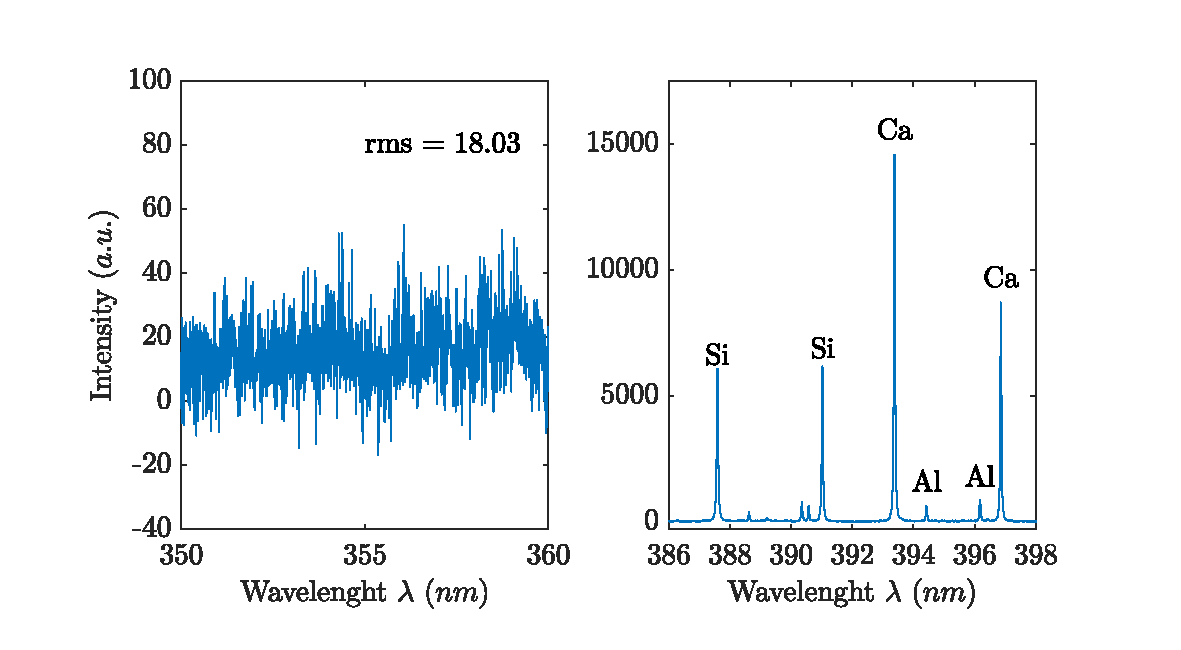
\includegraphics[width = \textwidth]{chapter_3/tests_graphs/test_NZK7_6mj_zoom.pdf} 
     \vspace*{-30pt}
    \caption{$\protect 6 \: mJ$ - (Left) Focus of on the noise. (Right) Focus on the $386 \: nm$ to $398 \: nm$ range.}
    \label{fig:test_NZK7_6mj_zoom}
 \end{figure}
Focusing on the part of the UV spectral range from $386 \: nm$ to $398 \: nm$, we see that the signal-to-noise ratio ($S.N.R$) is about 340 (the value is obtained by dividing the counts of the silicon I peak at $390.55 \: nm$ by the RMS of the noise calculated from $350 \: nm$ to $360 \: nm$).
\\
By increasing the energy value to $10 \: mJ$ we get:
\begin{figure}[H]
    \centering
    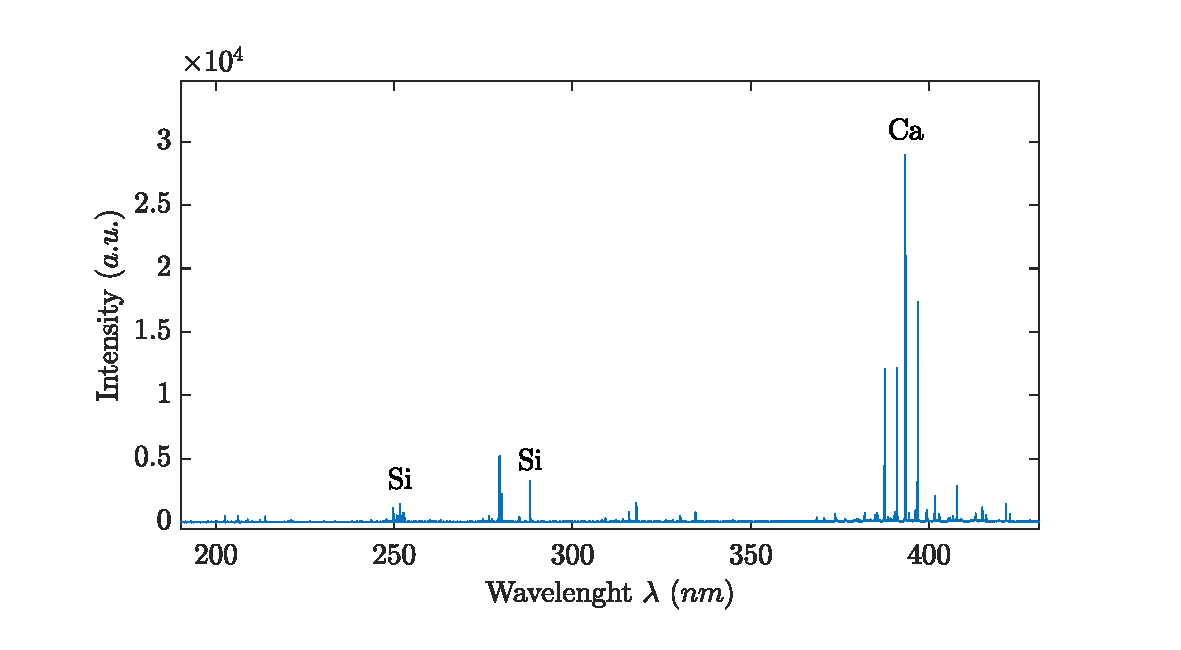
\includegraphics[width = \textwidth]{chapter_3/tests_graphs/test_NZK7_10mj.pdf} 
     \vspace*{-30pt}
    \caption{$\protect 10 \: mJ$ - Spectrum of NZK-7 glass.}
    \label{fig:test_NZK7_10mj}
\end{figure}
\begin{figure}[H]
    \centering
    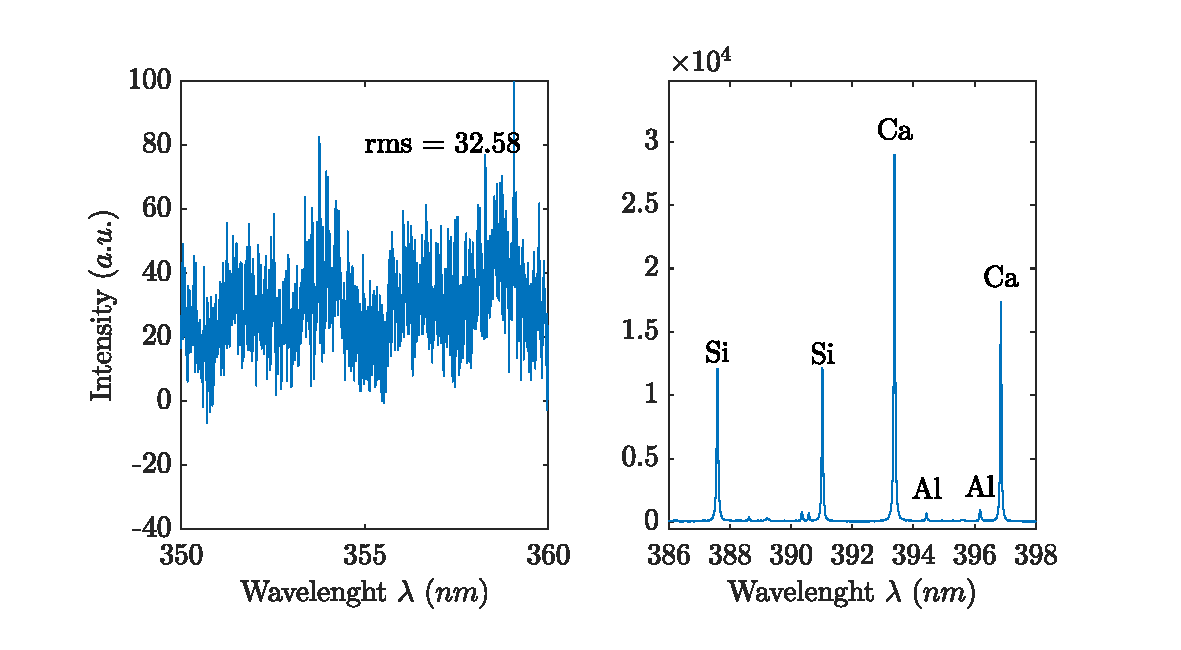
\includegraphics[width = \textwidth]{chapter_3/tests_graphs/test_NZK7_10mj_zoom.pdf} 
     \vspace*{-30pt}
    \caption{$\protect 10 \: mJ$ - (Left) Focus of on the noise. (Right) Focus on the $386 \: nm$ to $398 \: nm$ range.}
    \label{fig:test_NZK7_10mj_zoom}
 \end{figure}
Both the counts and the noise increased with the energy, but the overall $S.N.R.$ is higher, being around 370.
\\
Lastly, we tried $15 \: mJ$:
\begin{figure}[H]
    \centering
    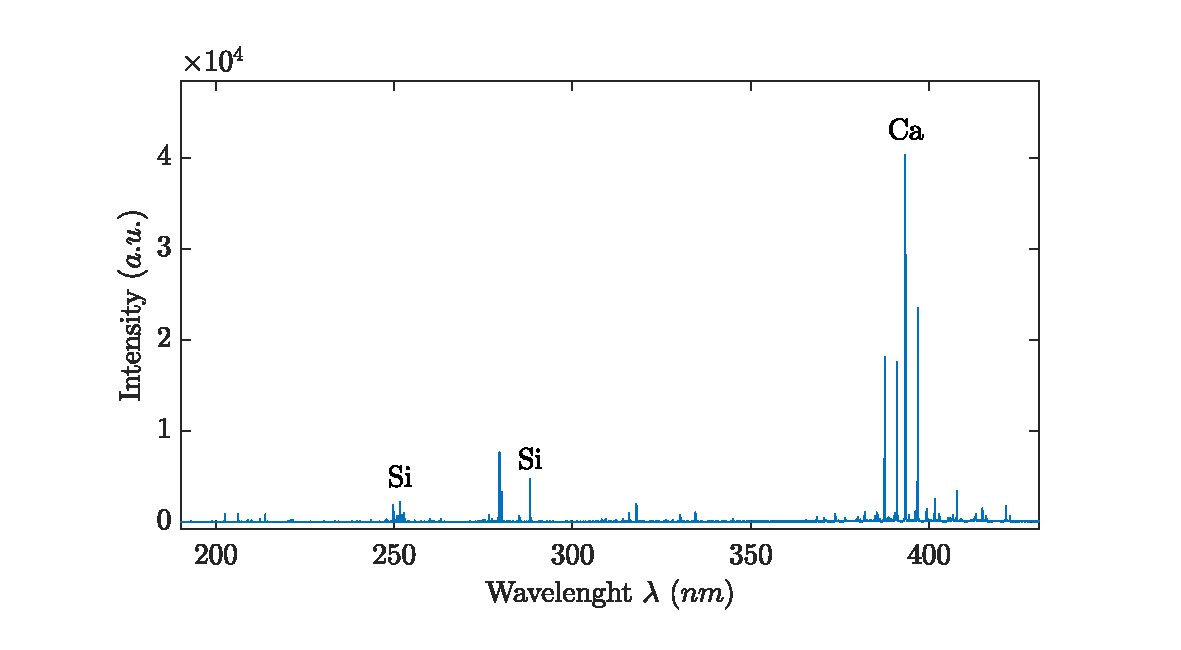
\includegraphics[width = \textwidth]{chapter_3/tests_graphs/test_NZK7_15mj.pdf} 
     \vspace*{-30pt}
    \caption{$\protect 15 \: mJ$ - Spectrum of NZK-7 glass.}
    \label{fig:test_NZK7_15mj}
\end{figure}
\begin{figure}[H]
    \centering
    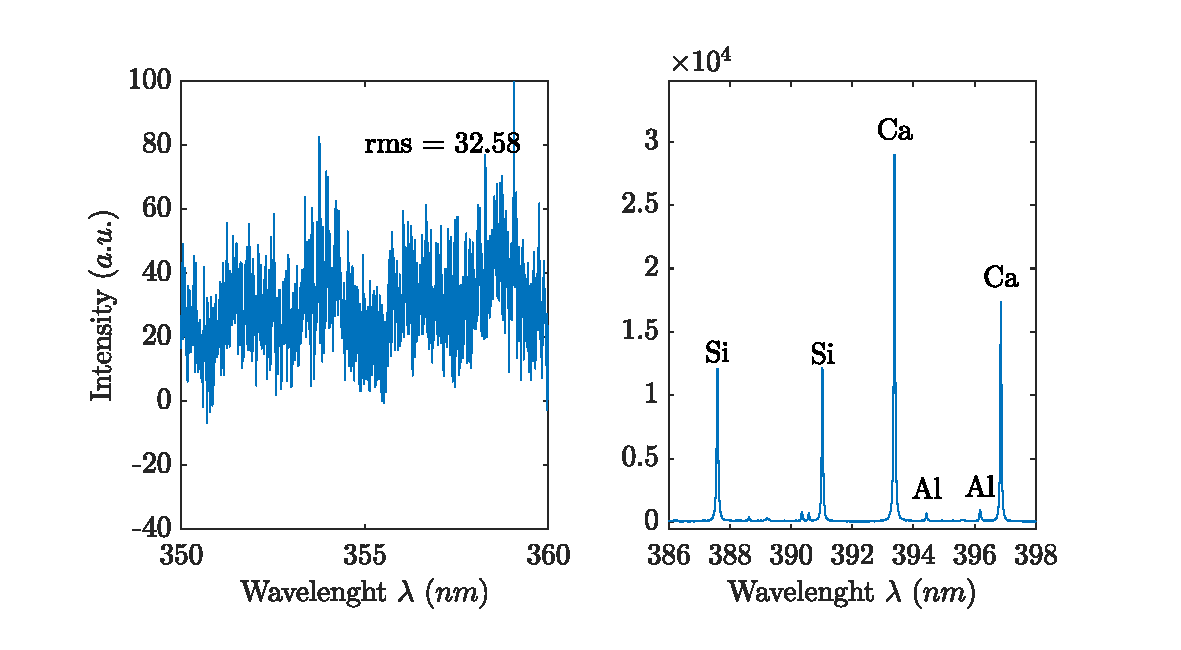
\includegraphics[width = \textwidth]{chapter_3/tests_graphs/test_NZK7_10mj_zoom.pdf} 
     \vspace*{-30pt}
    \caption{$\protect 15 \: mJ$ - (Left) Focus of on the noise. (Right) Focus on the $386 \: nm$ to $398 \: nm$ range.}
    \label{fig:test_NZK7_15mj_zoom}
 \end{figure}

For this value of the energy the $S.N.R.$ is still around 370, so we decided not to increase the energy anymore.
\\
In the end, therefore, we selected $15 \: mJ$ as the final value with which all the measurements have been carried out. 

\subsubsection{Gate Width and Time Delay}
\label{subsubsec:gate_width_delay}

To get the values that will give us the most comprehensive plasma spectrum, we decided to perform an analysis called “time evolution”, where the emission spectrum is recorded at various instants in the lifetime of the plasma. To ensure that the plasma parameters, such as electron density ($N_e$) and temperature ($T$), do not vary much within the measurements, in time evolution experiments, the gate width is always set to be equal to half the value of the time delay [jorg’s paper].
\\
The evolution was considered starting from a delay time of $0.5\: \mu s$, that corresponds to a gate width of $0.25 \: \mu s$, to a delay of $10 \: \mu s$ and $5 \: \mu s$ for the gate width.
\\
In Figure~\ref{fig:test_NZK7_time_evo_zoom} we have plotted the intensities of two silicon peaks in two different part of the spectral region for every spectrum of the time evolution. This was done to ensure that the differences measured were homogeneous along the whole frequency range.
\begin{figure}[H]
    \centering
    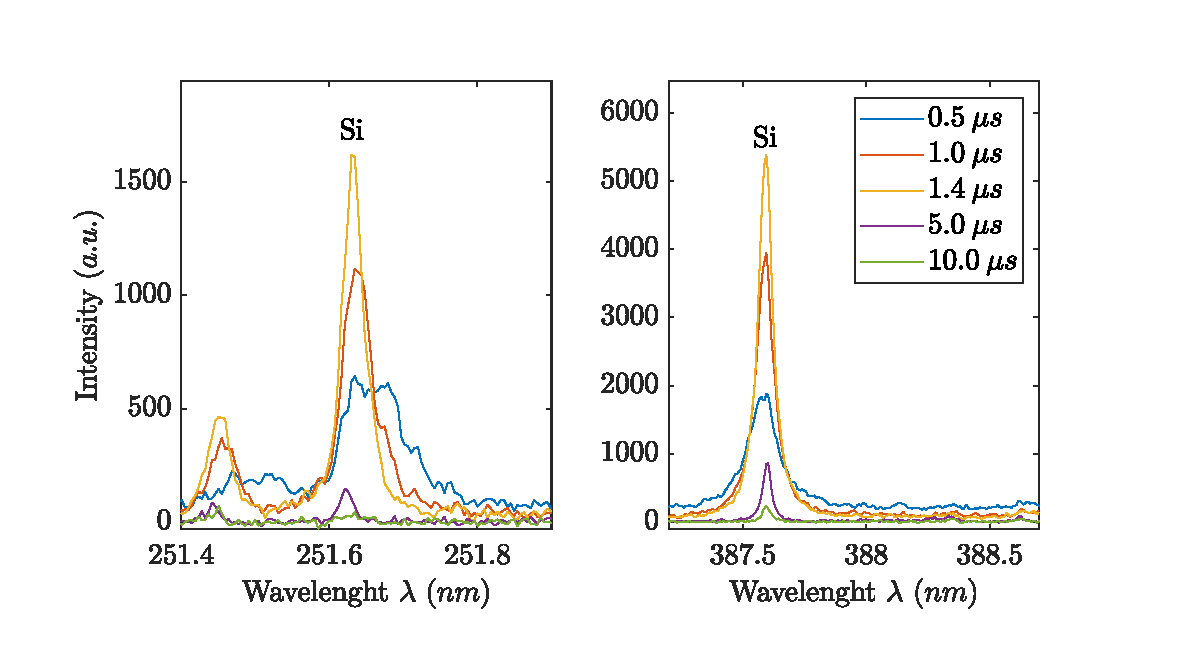
\includegraphics[width = \textwidth]{chapter_3/tests_graphs/test_NZK7_time_evo_zoom.pdf} 
    \vspace*{-30pt}
    \caption[Time evolution.]{Time evolution from $\protect 0.5\: \mu s$ to $10 \: \mu s$. (Left) Silicon peak at $251.63 \: nm$. (Right) Silicon peak at $387.53 \: nm$.}
    \label{fig:test_NZK7_time_evo_zoom}
 \end{figure}

 \begin{figure}[H]
    \centering
    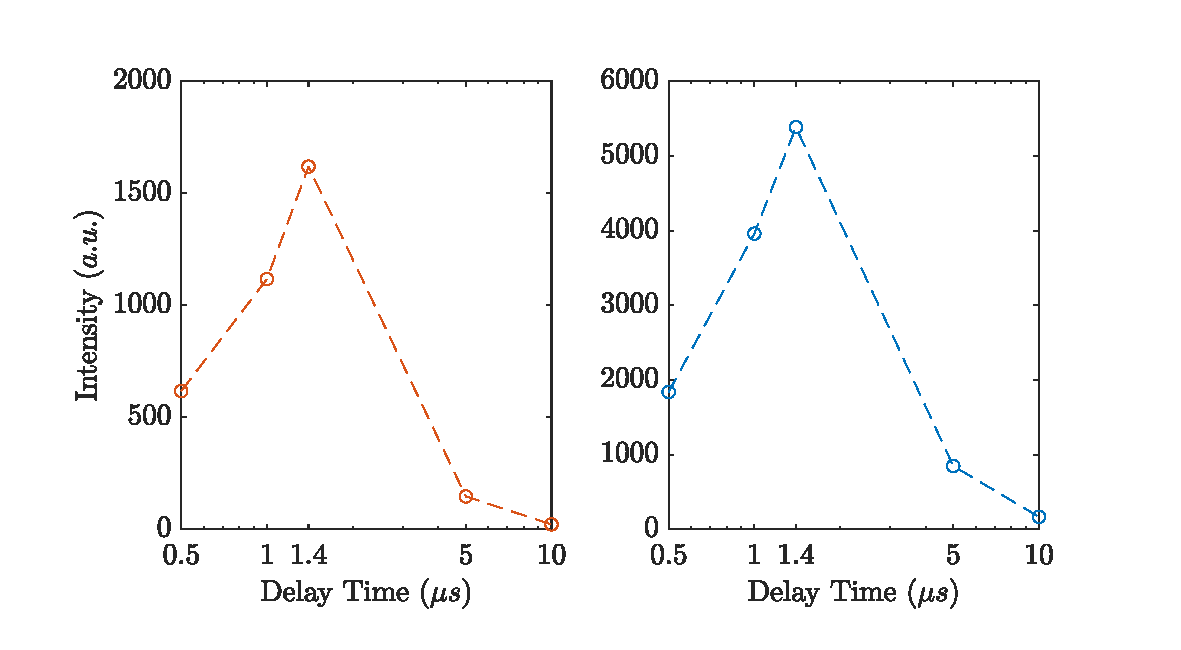
\includegraphics[width = \textwidth]{chapter_3/tests_graphs/time_evo_NZK7.pdf} 
    \vspace*{-30pt}
    \caption{Maximum intensity of the two peaks as a function of the delay time.}
    \label{fig:time_evo_NZK7}
 \end{figure}
In Figure~\ref{fig:time_evo_NZK7} is explicitly shown the maximum intensity of the two peaks as a function of the delay time. The highest intensity corresponds to a time of $1.4 \: \mu s$, and therefore this is the value that we have chosen for our measurements.
\\
Considering that the goal of our research involved finding contaminants that could be in low concentrations, for the gate width we chose a value of $12 \: \mu s$ to collect the highest amount of information possible from the measurements.

\subsubsection{Detector Gain}
\label{subsubsec:detector_gain}
The gain of the detector has been set to a value of 3000 because it is the default gain suggested by the manufacturer of the apparatus, and it is usually left unchanged.

\subsubsection{Number of Points per Measurement}
\label{subsubsec:number_points_mesurement}
Furthermore, all the analyses have been carried out taking the shots at 36 different points on the surface for each measurement. The points were separated by a distance of $150 \: \mu m$. The final spectrum is calculated as the average of the 36 different measurements, this is needed to reduce the intrinsic shot-to-shot variability that characterizes LIBS. 
\begin{figure}[H]
    \centering
    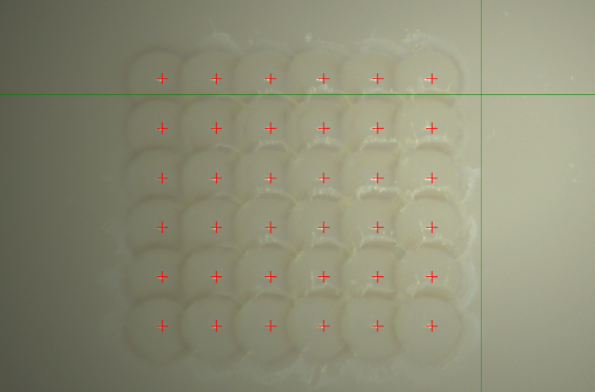
\includegraphics[width = 0.6\textwidth]{chapter_3/tests_graphs/grid_measurement.png} 
    %\vspace*{-30pt}
    \caption{Grid of measurements on the glass piece. }
    \label{fig:grid_measurement}
\end{figure}

\subsubsection{Number of Pulses per Measurement Point}
\label{subsec:number_pulses_mesurement}
Lastly, we investigated the influence on the spectrum related to the number of pulses per measurement. The LIBS apparatus gives the possibility of taking multiple laser shots at a single point on the surface, generating then the final spectrum as the average of the multiple measurements taken. This is a common way to easily increase the quality of data acquired and, usually, utilizing a large number of pulses is always preferred. The only downside in using multiple shots, other than increasing the measurement time, is that surface sensitivity is lost. In fact, each pulse ablates a portion of the material and increases the depth of the measurement.
\\ 
In our case, since contaminants are expected to diffuse only in a small region under the surface, we took a pure silica sample that had been polished for $2\:hrs$ and we took a series of consecutive measurements over the same spots to see after which number of pulses the impurities, such as aluminum, would not be detected anymore.
\\
The results are presented in Figure~\ref{fig:comparison_deep_scan}.
\begin{figure}[H]
    \centering
    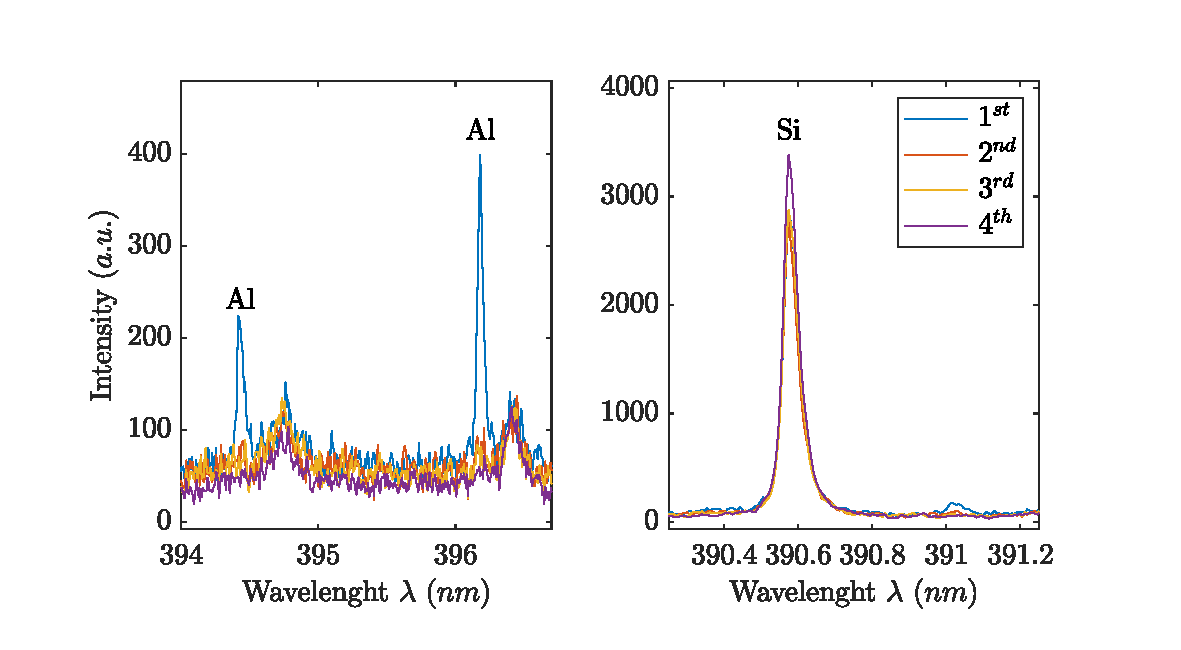
\includegraphics[width = \textwidth]{chapter_3/tests_graphs/test_NZK7_deep_scan_zoom.pdf} 
    \vspace*{-30pt}
    \caption[Comparison for consecutive pulses.]{Comparison for consecutive pulses on: (Left) Aluminum peaks around $\protect 395 \: nm$. (Right) Silicon peak at $\protect 390.6 \: nm$. The spectra are normalized with respect to the \ce{Si} peak at $\protect 288 \: nm$}
    \label{fig:comparison_deep_scan}
\end{figure}
On the left graph the most intense aluminum peaks are shown, while on the right, a nearby silicon peak is shown as a comparison. It is clear that the presence of aluminum cannot be detected after the first laser pulse, underlining its presence only on the surface. 
\\
This means that, for all our measurements, we could not perform more than one pulse. This was not ideal both for the statistical quality of the data, and for the risk of external contamination of the samples impacting on the experiment. In fact, errors in cleaning or handling of the sample, that could be averaged out by multiple pulses, could give instead a higher contribution.
\\
As a summary, the parameters chosen were:
\begin{itemize}
\item Laser energy: $15 \: mJ$
\item Delay time: $1.4 \: \mu s$
\item Gate width: $12 \: \mu s$
\item Detector gain: 3000
\item Number of pulses: 1
\end{itemize}

\subsection{Analysis Workflow}
\label{subsec:analysis_workflow}
Analysis of LIBS data is a crucial step that can be carried out both under a qualitative and a quantitative profile. Qualitative analysis requires much less time and commitment and can be carried out by a simple visual comparison of the measured spectra. It is usually employed when a fast result is needed. However, when a more sophisticated and precise result is sought, quantitative analysis can be utilized to calculate the relative concentrations of the different elemental species that compose the sample.
\\
In quantitative analyses, standard samples are usually utilized to calibrate the LIBS measurements. These are pellets prepared with well-defined and known element composition ratios.
\\
The technique that we exploited, however, is called “Calibration-free LIBS” and does not require the use of any standard for calibration. It requires instead the knowledge of some technical properties of the apparatus, as the apparatus response over the whole spectral range and the intrinsic width of the spectrometer.
\begin{figure}[H]
    \centering
    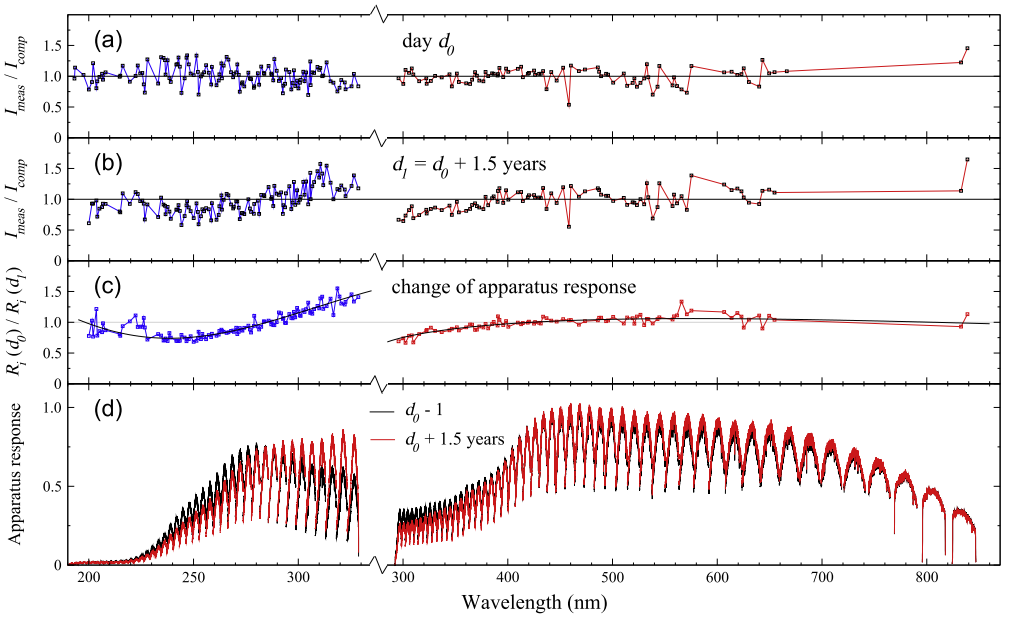
\includegraphics[width = \textwidth]{chapter_3/analysis_workflow/apparatus_response.png} 
    %\vspace*{-30pt}
    \caption{In the bottom plot of the figure it is shown an example of a typical apparatus response. }
    \label{fig:apparatus_response}
\end{figure}
In addition, for analysis to be valid, the measured plasma must satisfy the LTE condition.
\\
The analysis of the data has been carried out through the use of a program called: “Analyze LTE Plasma Spectra” (Ver. 2.6.6) or “LTEspec” in short.
\\
This application is hosted on the servers of the LP3 laboratories of the Université d’Aix-Marseille. A detailed explanation of the working principle of the algorithm behind the software can be found here [Jorg’s Paper].
\\
In the next section we will describe the passages needed to obtain the quantitative results that will be presented in the later sections.
\subsubsection{Spectra Preparation}
\label{subsubsec:spectra_preparation}
The first step is the preparation of the spectrum. The LIBS apparatus was used to measure two separate spectra, UV and visible, for each analyzed sample. To induce the exact same plasma conditions for the two ranges, we always maintained the same laser and detector parameters.


\begin{figure}[H]
    \centering
    \subfloat[UV spectrum. \label{fig:uv_non_corr}]{
        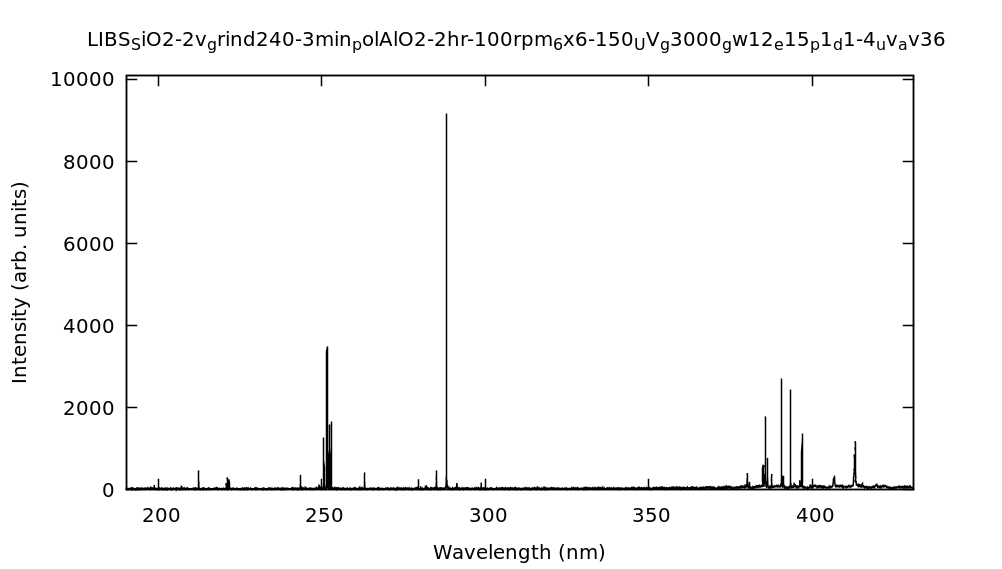
\includegraphics[width = 0.45\textwidth]{chapter_3/analysis_workflow/Uv.png}
    }
    \quad
    \subfloat[Vis Spectrum. \label{fig:vis_non_corr}]{
        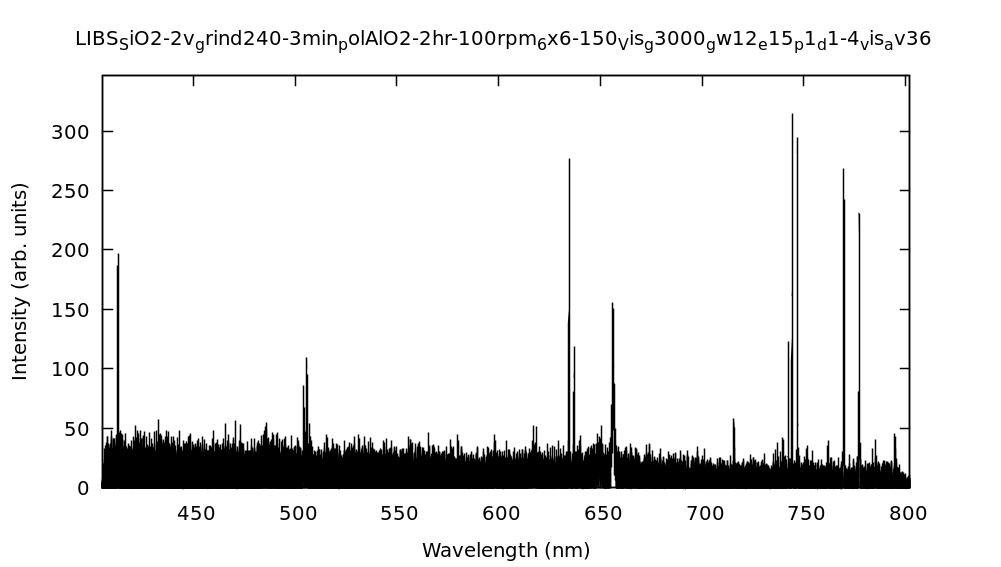
\includegraphics[width = 0.45\textwidth]{chapter_3/analysis_workflow/Vis.png}
    }
    \caption{Spectra before the correction. }
    \label{fig:spectra_before_corr}
\end{figure}




The first action we need to undertake is to connect the two graphs in order to obtain only one single spectrum comprising the whole spectral range, that spans from 190 to 800 nm. The procedure, though, is not trivial. Due to the different sensitivities of the two spectrometers, the two measured spectra have a quite different intensity reading and signal to noise ratio. In particular, the visible spectrum presents a much lower photon count.
\\ 
Thanks to the fact that the two measured spectra share a portion of the wavelength range, specifically, from 405 to 430 nm, the analysis program will use the two silicon peaks present in this region to normalize the two spectra, rescaling the intensity of the visible one. The usual rescale factor for our measurements is around 6. The visible spectrum must be therefore multiplied by 6 to match the intensities of the peaks between the UV and visible data.
\\
Here are the photos of before and after the scaling of the two spectra in the range from 400 to 430 nm, where it can be seen that the peak present at, roughly, 412 nm has been used to fit the visible (red) spectrum to the intensity of the UV (black) spectrum.


\begin{figure}[H]
    \centering
    \subfloat[UV spectrum. \label{fig:uv_vis_non_corr}]{
        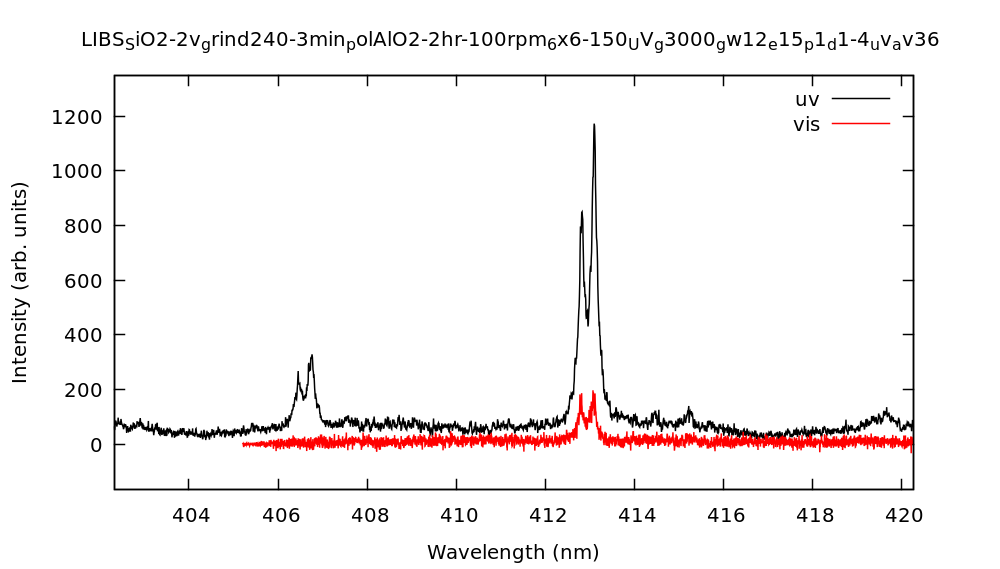
\includegraphics[width = 0.45\textwidth]{chapter_3/analysis_workflow/UvVis not corrected.png}
    }
    \quad
    \subfloat[Vis Spectrum. \label{fig:uv_vis_corr}]{
        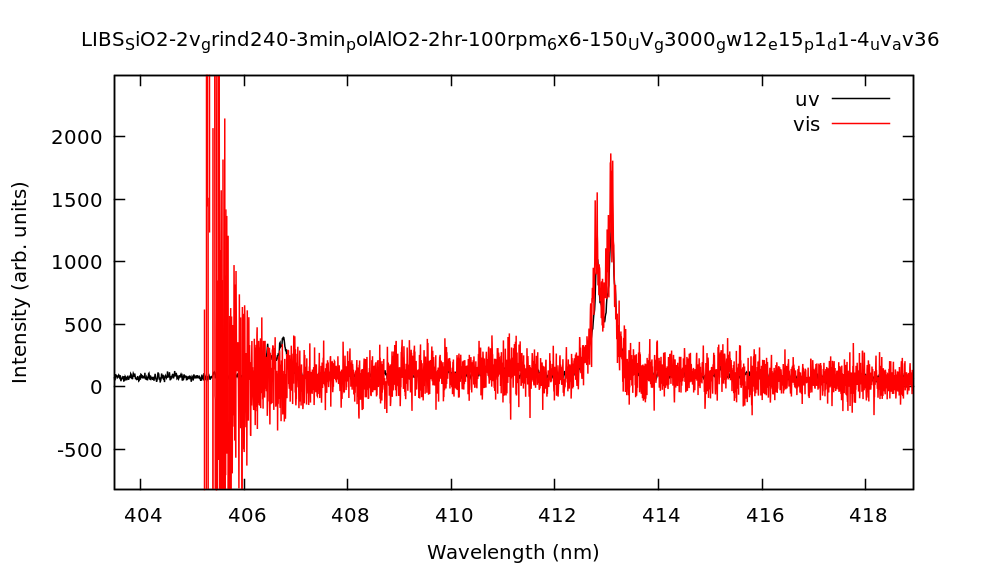
\includegraphics[width = 0.45\textwidth]{chapter_3/analysis_workflow/UvVis corrected.png}
    }
    \caption{The merging point of the two spectra before and after applying the correction and the scale factor. }
    \label{fig:spectra_mergin_point}
\end{figure}


\begin{figure}[H]
    \centering
    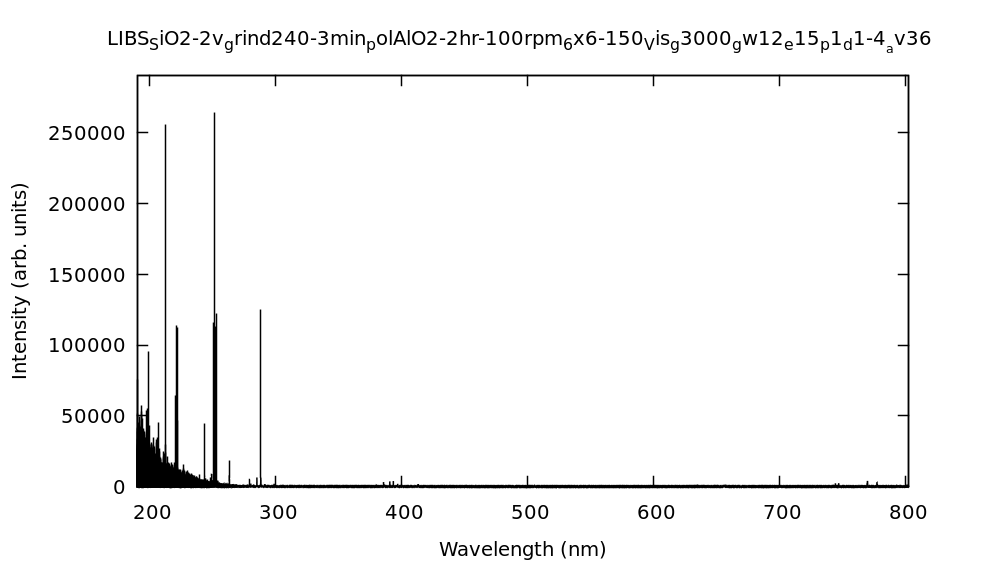
\includegraphics[width = \textwidth]{chapter_3/analysis_workflow/UvVis merged.png} 
    %\vspace*{-30pt}
    \caption{The final spectrum (UV + Vis) after the merging. }
    \label{fig:merged_sepctrum}
\end{figure}


During the merging process, the rescaling factor is not the only applied parameter. As already mentioned, the apparatus itself has a spectral response that is not homogeneous, that varies across the whole range. The spectral response had been measured, and the program can apply the corresponding correction UV and visible spectra. Lastly, other machine-dependent corrections are applied like the apparatus spectral width and the wavelength calibration are applied.

\subsubsection{Spectrum Analysis}
\label{subsubsec:spectrum_analysis}
Once the complete spectrum has been derived, the proper quantitative analysis can start. 

\paragraph{Electron density and Optical Thickness}
\label{par:electron_density_opt_thick}
The first step in the plasma diagnostic process is to select a reference intensity peak from which Stark and Doppler broadening parameters are measured; these are in fact the dominant mechanisms of spectra line broadening in laser induced plasmas [Paper’s 36][maybe cite the chapter of the thesis]. Those values are then used to measure the plasma optical thickness.
\\
Under the assumption of a linear dependance of the Stark width and shift with the electron density, the latter can be derived by measuring the width of a line with a significant Stark shift. A common choice for this estimation is the H-$\alpha$ lines at $656.28\:nm$ [Paper].
\\
In our case the Si I transition at $390.55 \: nm$ has been chosen for both the measurements.
\paragraph{Plasma Temperature}
\label{par:plasma_temperature}
After the determination of the electron density, the plasma temperature is derived from the Boltzmann plot (Chapter~\ref{subsubsec:thermodynamic_eq}) regarding the \ce{Si I} $390.55\:nm$ line and the ionized \ce{Si II} doublet at 385.60 and $386.26\:nm$ [Paper].


\begin{figure}[H]
    \centering
    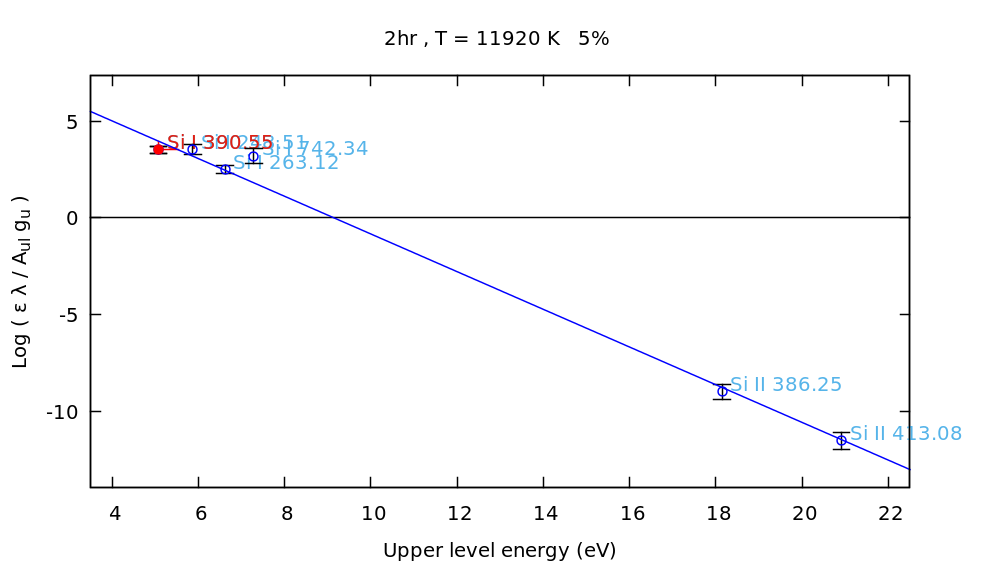
\includegraphics[width = \textwidth]{chapter_3/analysis_workflow/Boltzmann plot SI.png} 
    %\vspace*{-30pt}
    \caption{Boltzmann plot used to estimate the plasma temperature. }
    \label{fig:boltzmann_plot}
\end{figure}


\paragraph{Plasma Parameter}
\label{par:plasma_parameter}
The size of the plasma is derived from interpolating the laser settings present in the metadata of the file, with experimental measurements done at the apparatus, where the size of the plasma was measured over its whole lifetime using a high-speed camera.
\paragraph{Element Search and Relative Concentration Calculation}
Once an approximate value of the electron density Ne, the plasma temperature T and the optical thickness of the plasma have been measured, it is possible to carry out an automatic search of the element species that are present in the plasma. 
The spectral lines used for the analysis are selected according to the following criteria [Paper]:
\begin{itemize}
    \item The overlapping of spectral lines has to be avoided.
    \item The emission intensity must be large enough in order to have a large signal to noise ratio for the selected peaks.
    \item The lines must have a weak enough optical thickness to have a significant correlation between elemental concentration and line intensity
\end{itemize}

Here are presented some plots of the elements’ measured lines (in black), versus the expected emission based on the calculated plasma parameters and estimated concentration (in red). The more the fitting is precise, the more the plasma parameters represent valid approximations of the real values.

\begin{figure}[H]
    \centering
    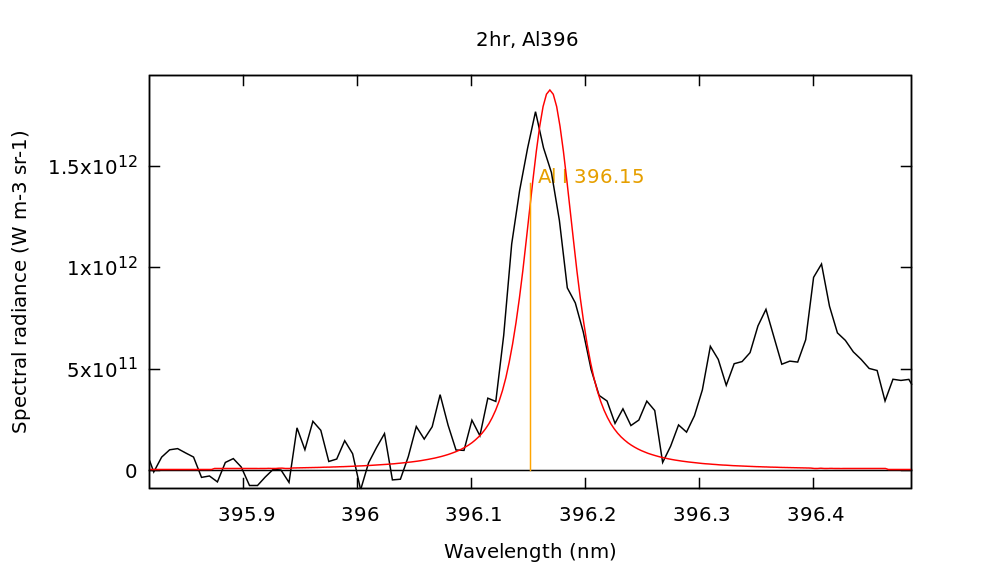
\includegraphics[width = 0.8\textwidth]{chapter_3/analysis_workflow/Al I line 396.png} 
    %\vspace*{-30pt}
    \caption{Aluminum line at $\protect 396.15 \:nm$}
    \label{fig:aluminum_line_lte}
\end{figure}
\begin{figure}[H]
    \centering
    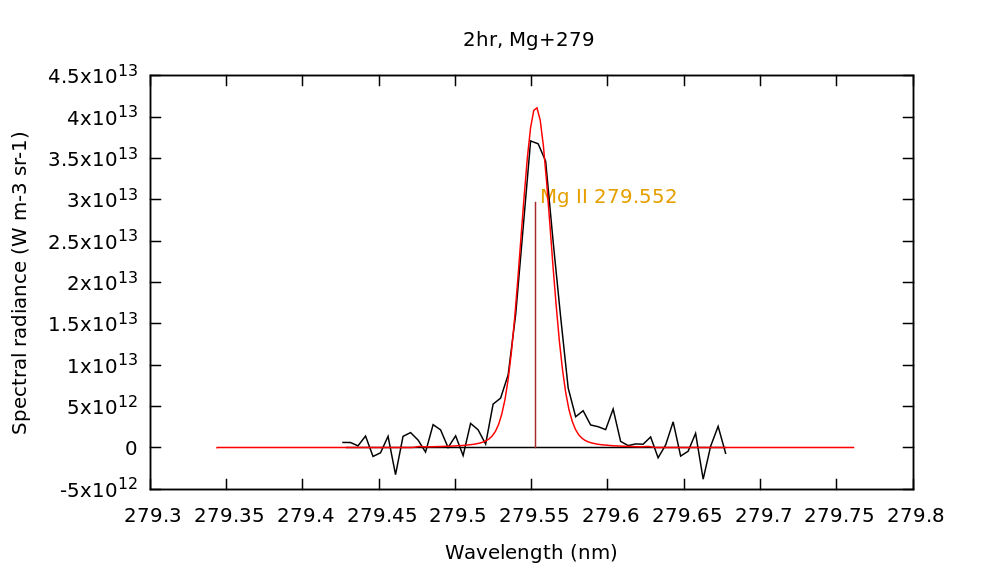
\includegraphics[width = 0.8\textwidth]{chapter_3/analysis_workflow/Mg II line 279.png} 
    %\vspace*{-30pt}
    \caption{Magnesium line at $\protect 279.55 \:nm$ }
    \label{fig:magnesium_line_lte}
\end{figure}
\begin{figure}[H]
    \centering
    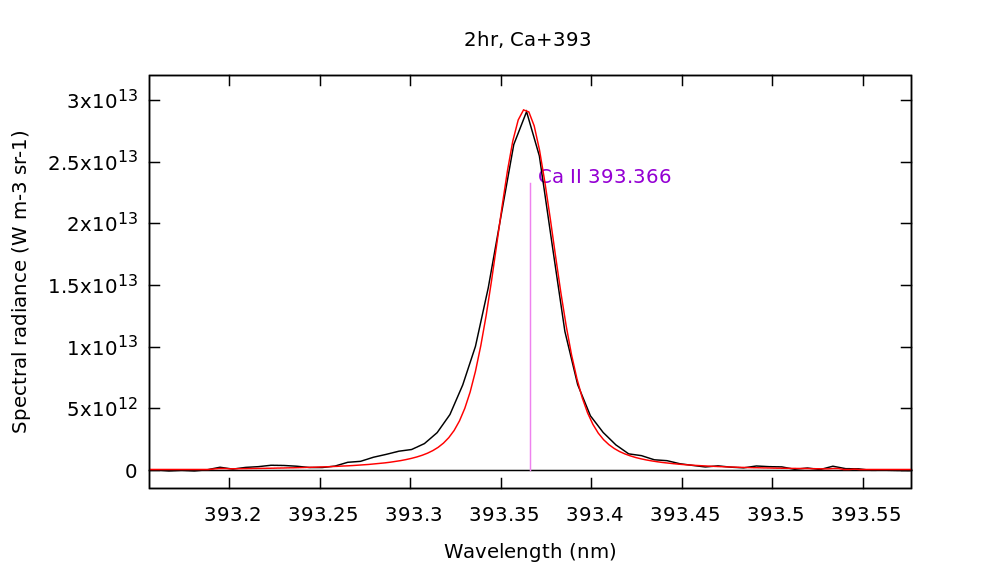
\includegraphics[width = 0.8\textwidth]{chapter_3/analysis_workflow/Ca II line 393.png} 
    %\vspace*{-30pt}
    \caption{Calcium line at $\protect 393.37 \:nm$ }
    \label{fig:calcium_line_lte}
\end{figure}

After the elements have been identified, all the plasma parameters are derived again, along with the relative concentrations of the elements. 

\subsubsection{Issues with Oxygen}
\label{subsubsec:oxygen_issues}

Particular attention must be paid with respect to the measurement of the oxygen concentration. In pure fused silica glass (\ce{SiO2}), oxygen makes up for most of the species in the glass composition, since its stoichiometric contribution is of about 2/3, or roughly 68\% of the total number of atoms. Oxygen atoms are characterized by large gaps between energy levels of the exited states, for this reason, for most the oxygen species, the thermodynamic equilibrium is hardly established [paper jorg] and therefore the measured lines cannot be use in the calibration-free method.
\\
This issue is even more noticeable when carrying out LIBS measurements in ambient air, like in our case, because oxygen is also present in the air surrounding the target sample and therefore, the measured emission is higher relative to the expected one from the real composition of the sample. 
\\
Under this condition, the standard procedure is to manually set the relative concentration of oxygen to be equal to the theoretical stoichiometric fraction. For our purposes, the concentration of oxygen is not a relevant quantity and therefore this approximation should not impact the other measurements.













\section{Polishing}
\label{Polishing}
Ensuring a uniform and correct polishing of the glass samples was one of the main concerns of our project. The procedure had to be reproducible and consistent between different runs, in order to introduce the least amount of non-controllable variables and to isolate the effect of the parameters that we were investigating.
\\
In addition, some of the samples were processed even up to consecutive hours, so a partial automatization of the workflow had to be done.
\subsection{Description of the Polishing Apparatus}
\label{subsec:description_polish_apparatus}
In this section, we will briefly describe the primary instrumentation we employed for glass processing.

\subsubsection{Polishing Machine}
\label{subsubsec:polishing_machine}
The polishing machine is one of the most important components.
\\
For our purposes, we employed a model manufactured by the company Buehler, specifically the Ecomet 4. The machine was utilized both to grind and polish all the analyzed glass samples. 
\begin{figure}[H]
    \centering
    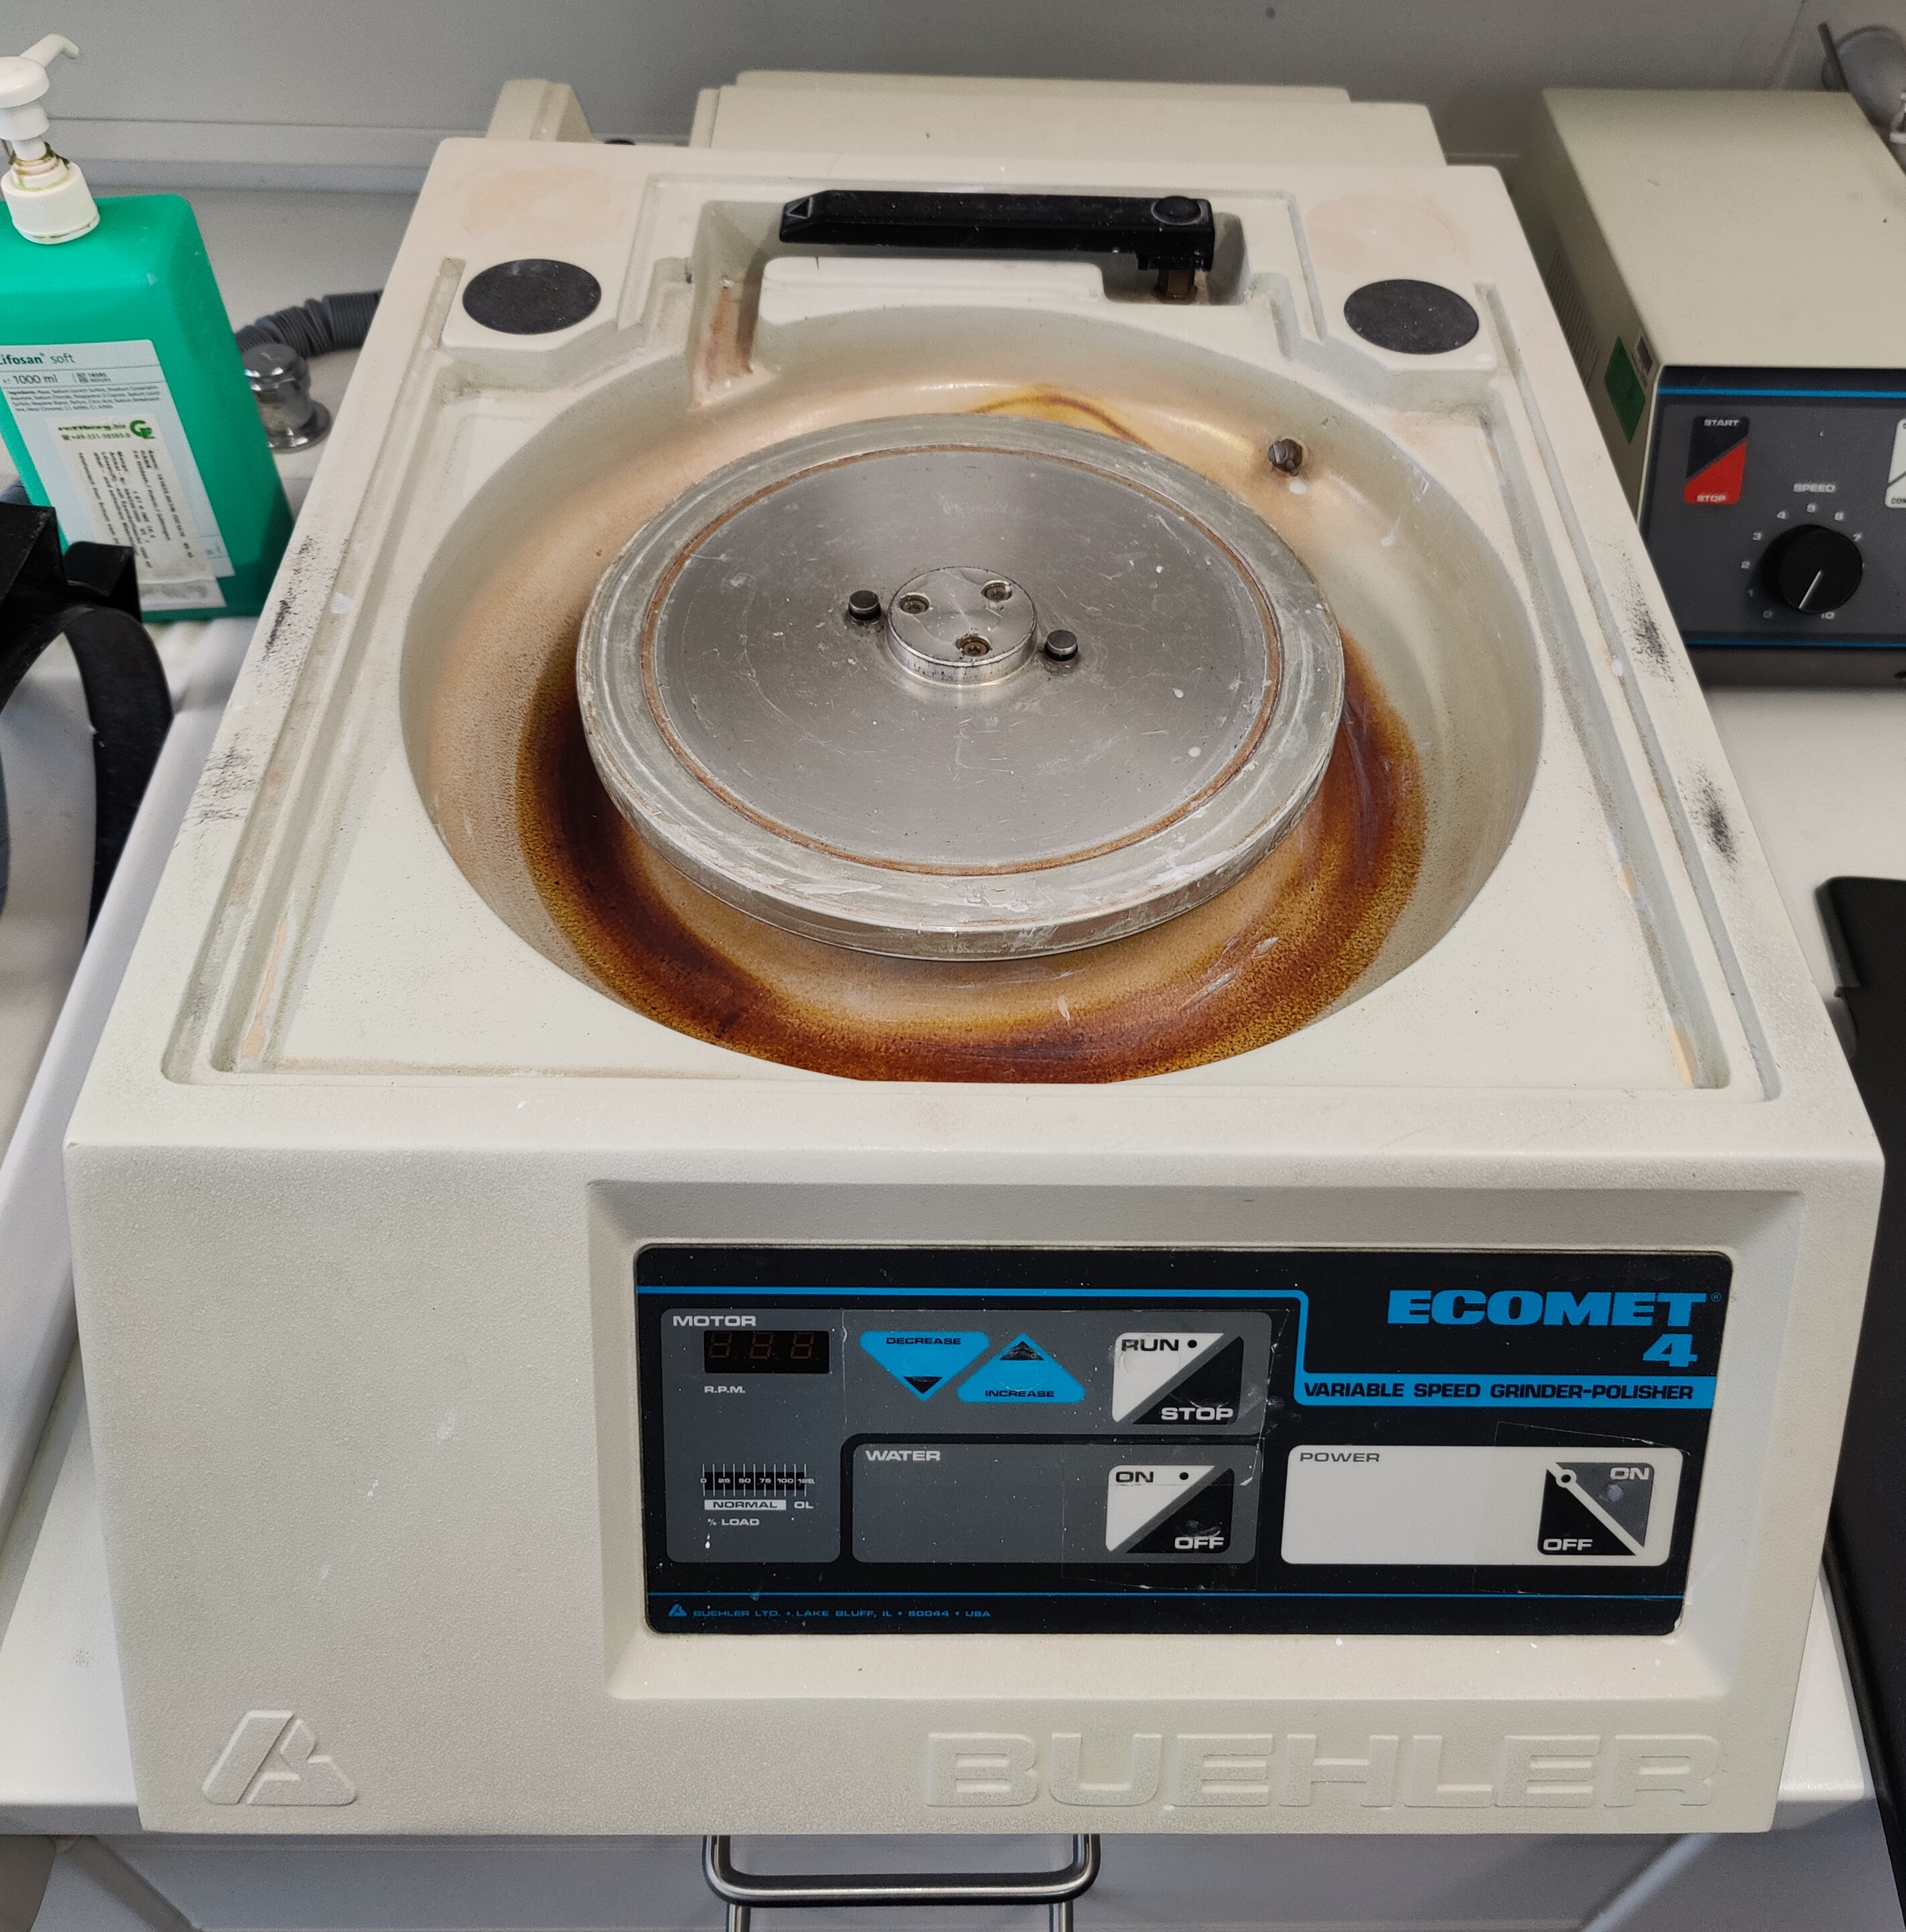
\includegraphics[width = 0.5\textwidth]{chapter_3/polish_setup_graphs/ecomet_4.jpg} 
    %\vspace*{-30pt}
    \caption{Photograph of the Ecomet 4.}
    \label{fig:ecomet_4}
\end{figure}
The apparatus is composed of a rotating platen on which either grinding paper or polishing cloth can be installed. The revolutions per minute (RPMs) of the platen could be easily modified to a specific value and, in addition, a constant source of tap water could be turned on. The machine is completely manual, meaning that the user needs to manually apply a down-pressing force upon the glass, while the platen is turning, to ensure correct contact between the platen itself and the sample.
\\
As anticipated before, long sessions of polishing needed to be carried out. To simplify the procedure and to reduce the influence of human error, an automatic way of holding and pressuring the sample was implemented.

\subsubsection{Sample Holder}
\label{subsubsec:sample_holder}
A simple block of machined aluminum, with carved out holes of the same size as the glass samples ($1\: cm$ of diameter and $2\: mm$ of thickness), was employed to hold the glass in place during both grinding and polishing. Using some small metal washers as spacers, it was possible to make the samples stick out from the holder, allowing only for their surface to make contact with the polishing pad. 

\begin{figure}[H]
    \centering
    \subfloat[Design of the holder. a) Holder, b) Washers, c) Glas samples, d) Polishing surface. \label{fig:holder_design}]{
        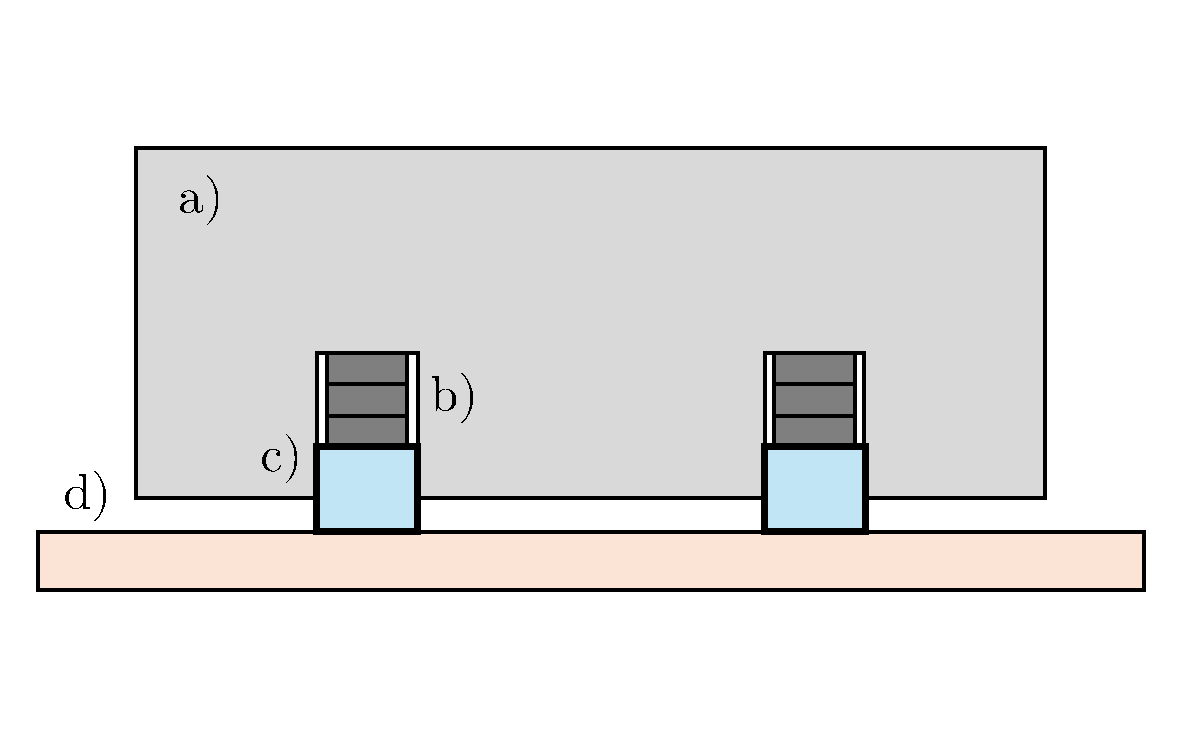
\includegraphics[scale=0.4]{chapter_3/polish_setup_graphs/holder_design.pdf}
    }
    \quad
    \subfloat[Photo of the holder. \label{fig:holder_photo}]{
        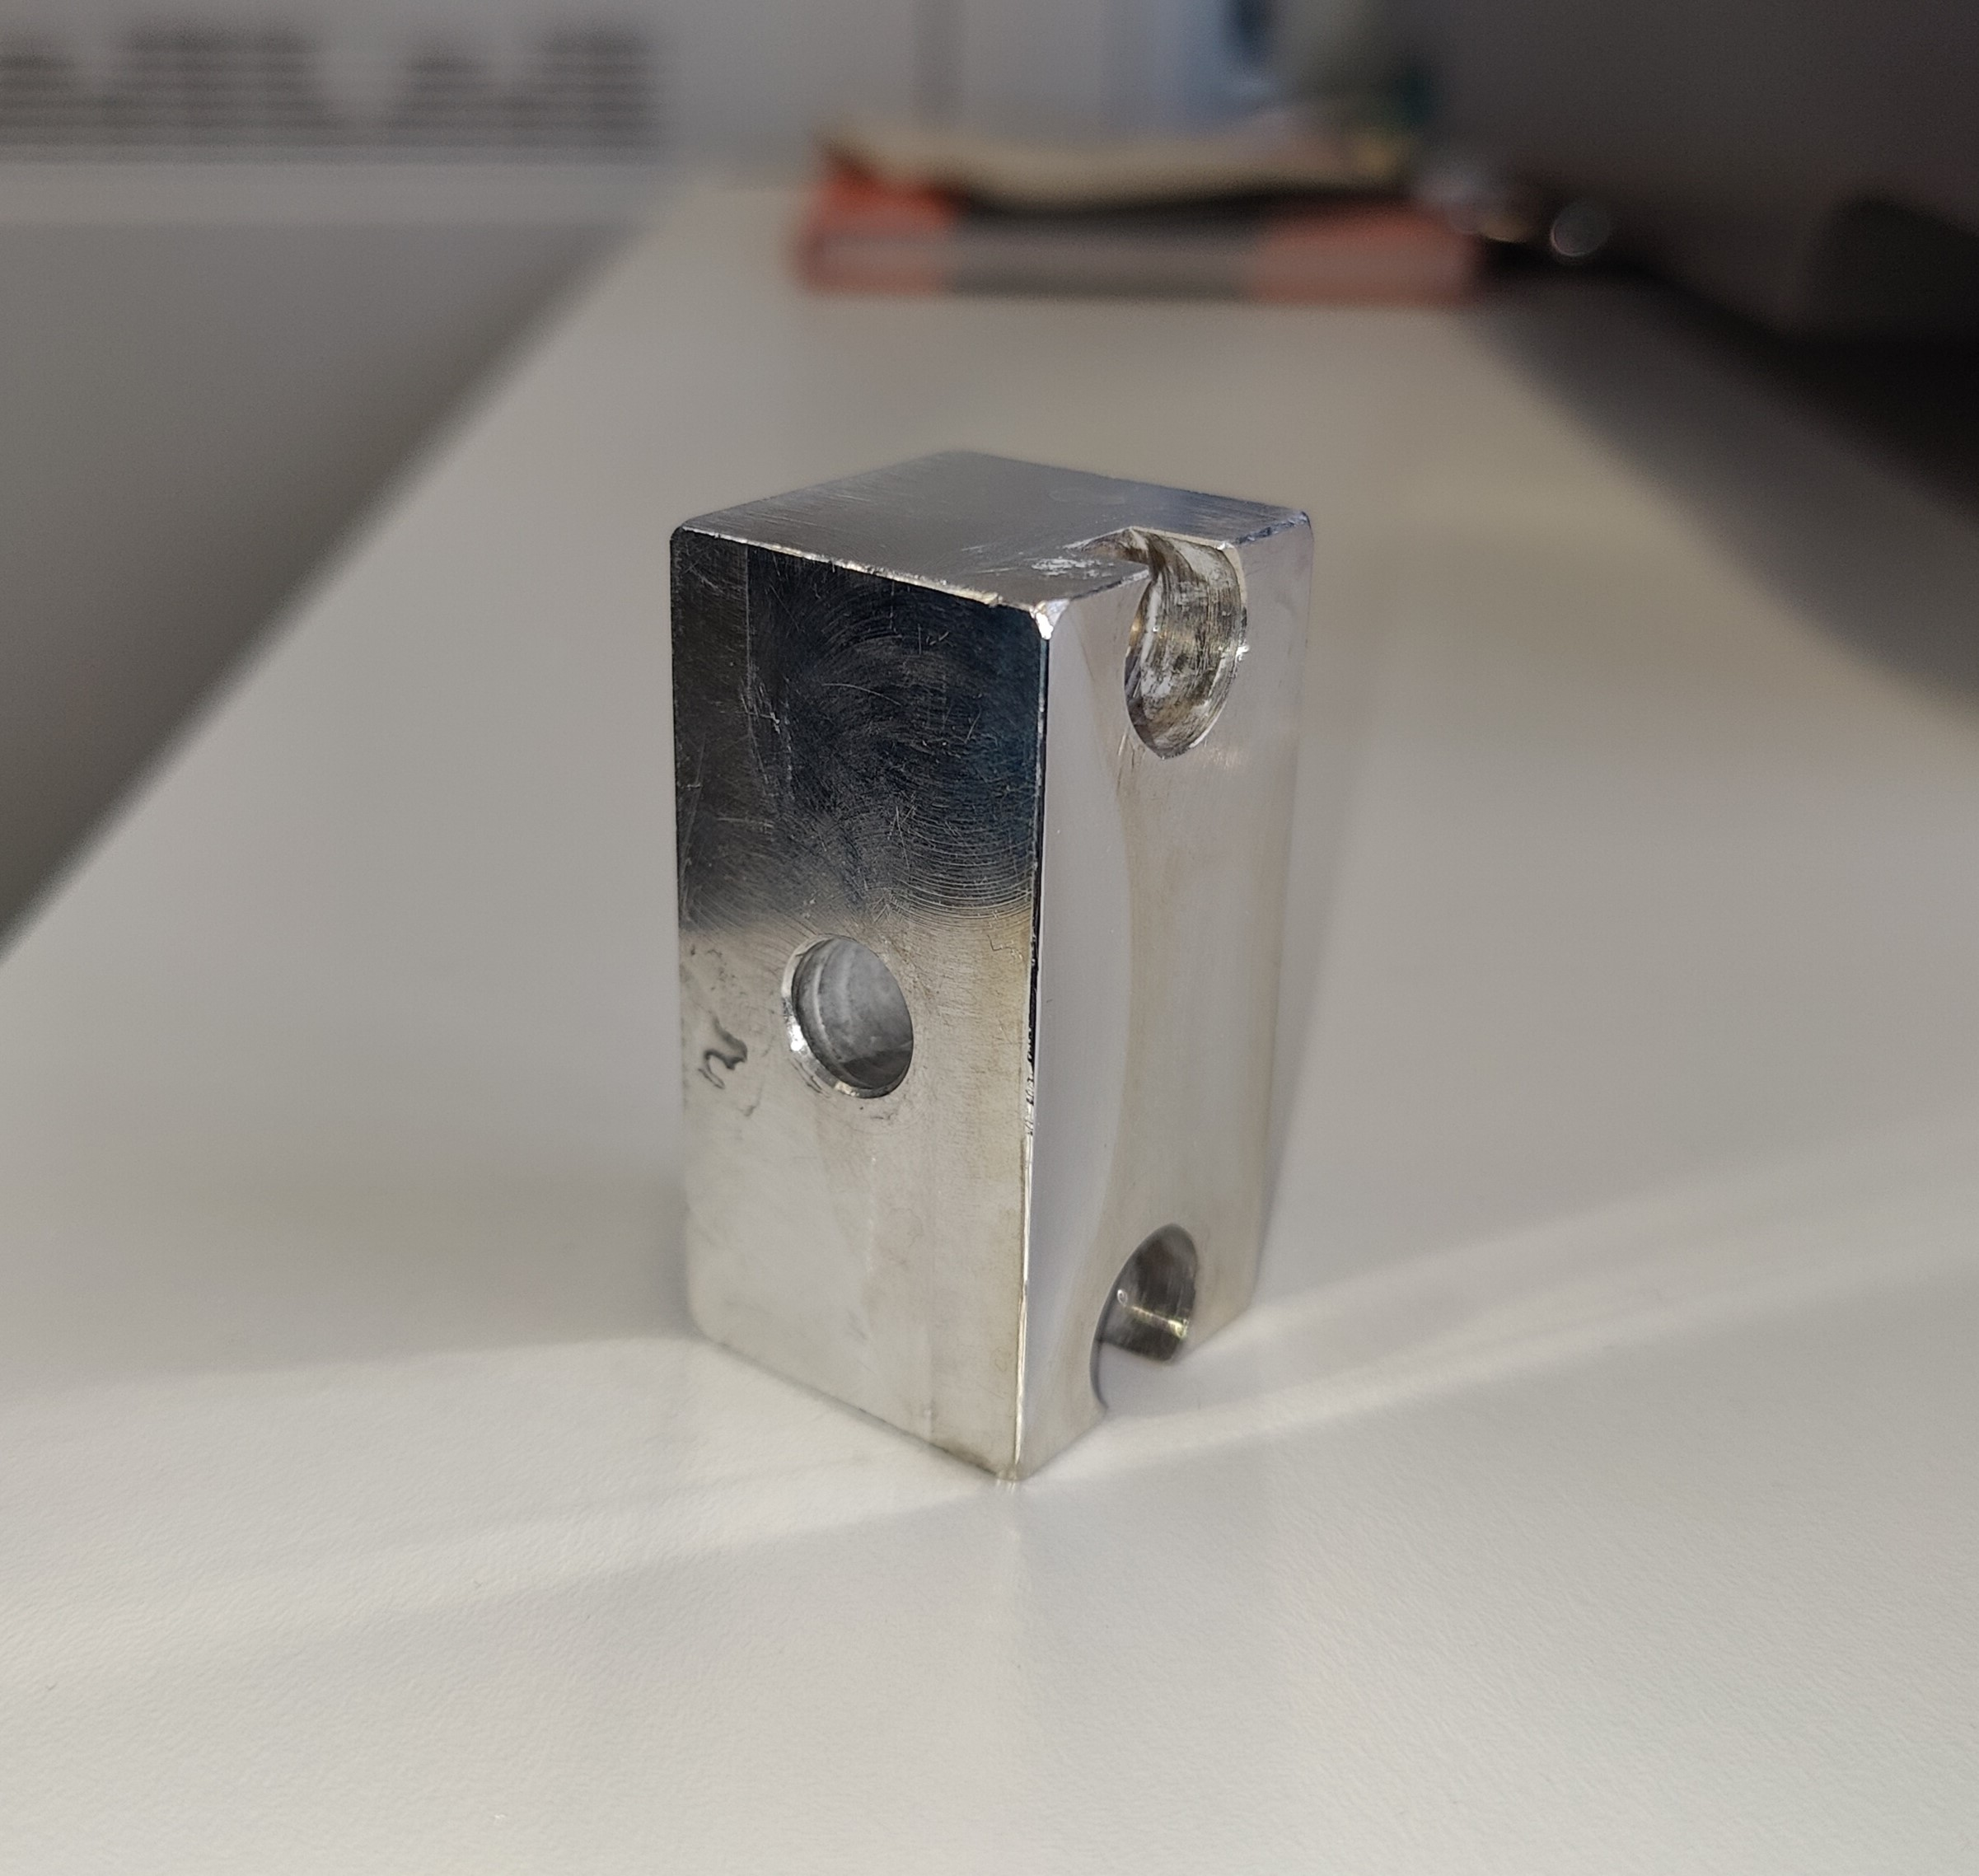
\includegraphics[scale=0.07]{chapter_3/polish_setup_graphs/aluminum_holder.jpg}
    }
    \caption{Aluminum holder for the glass samples. }
    \label{fig:holder}
\end{figure}
The aluminum block, while holding the glass samples, was held firm by another custom manufactured metal element, shown in Figure~\ref{fig:aluminum_structure}, that was anchored to the polishing machine frame. In this way, during both the grinding and the polishing phases, the holder could resist the friction forces caused by the 
platen rotation, maintaining fixed the sample position during the process.
\begin{figure}[H]
    \centering
    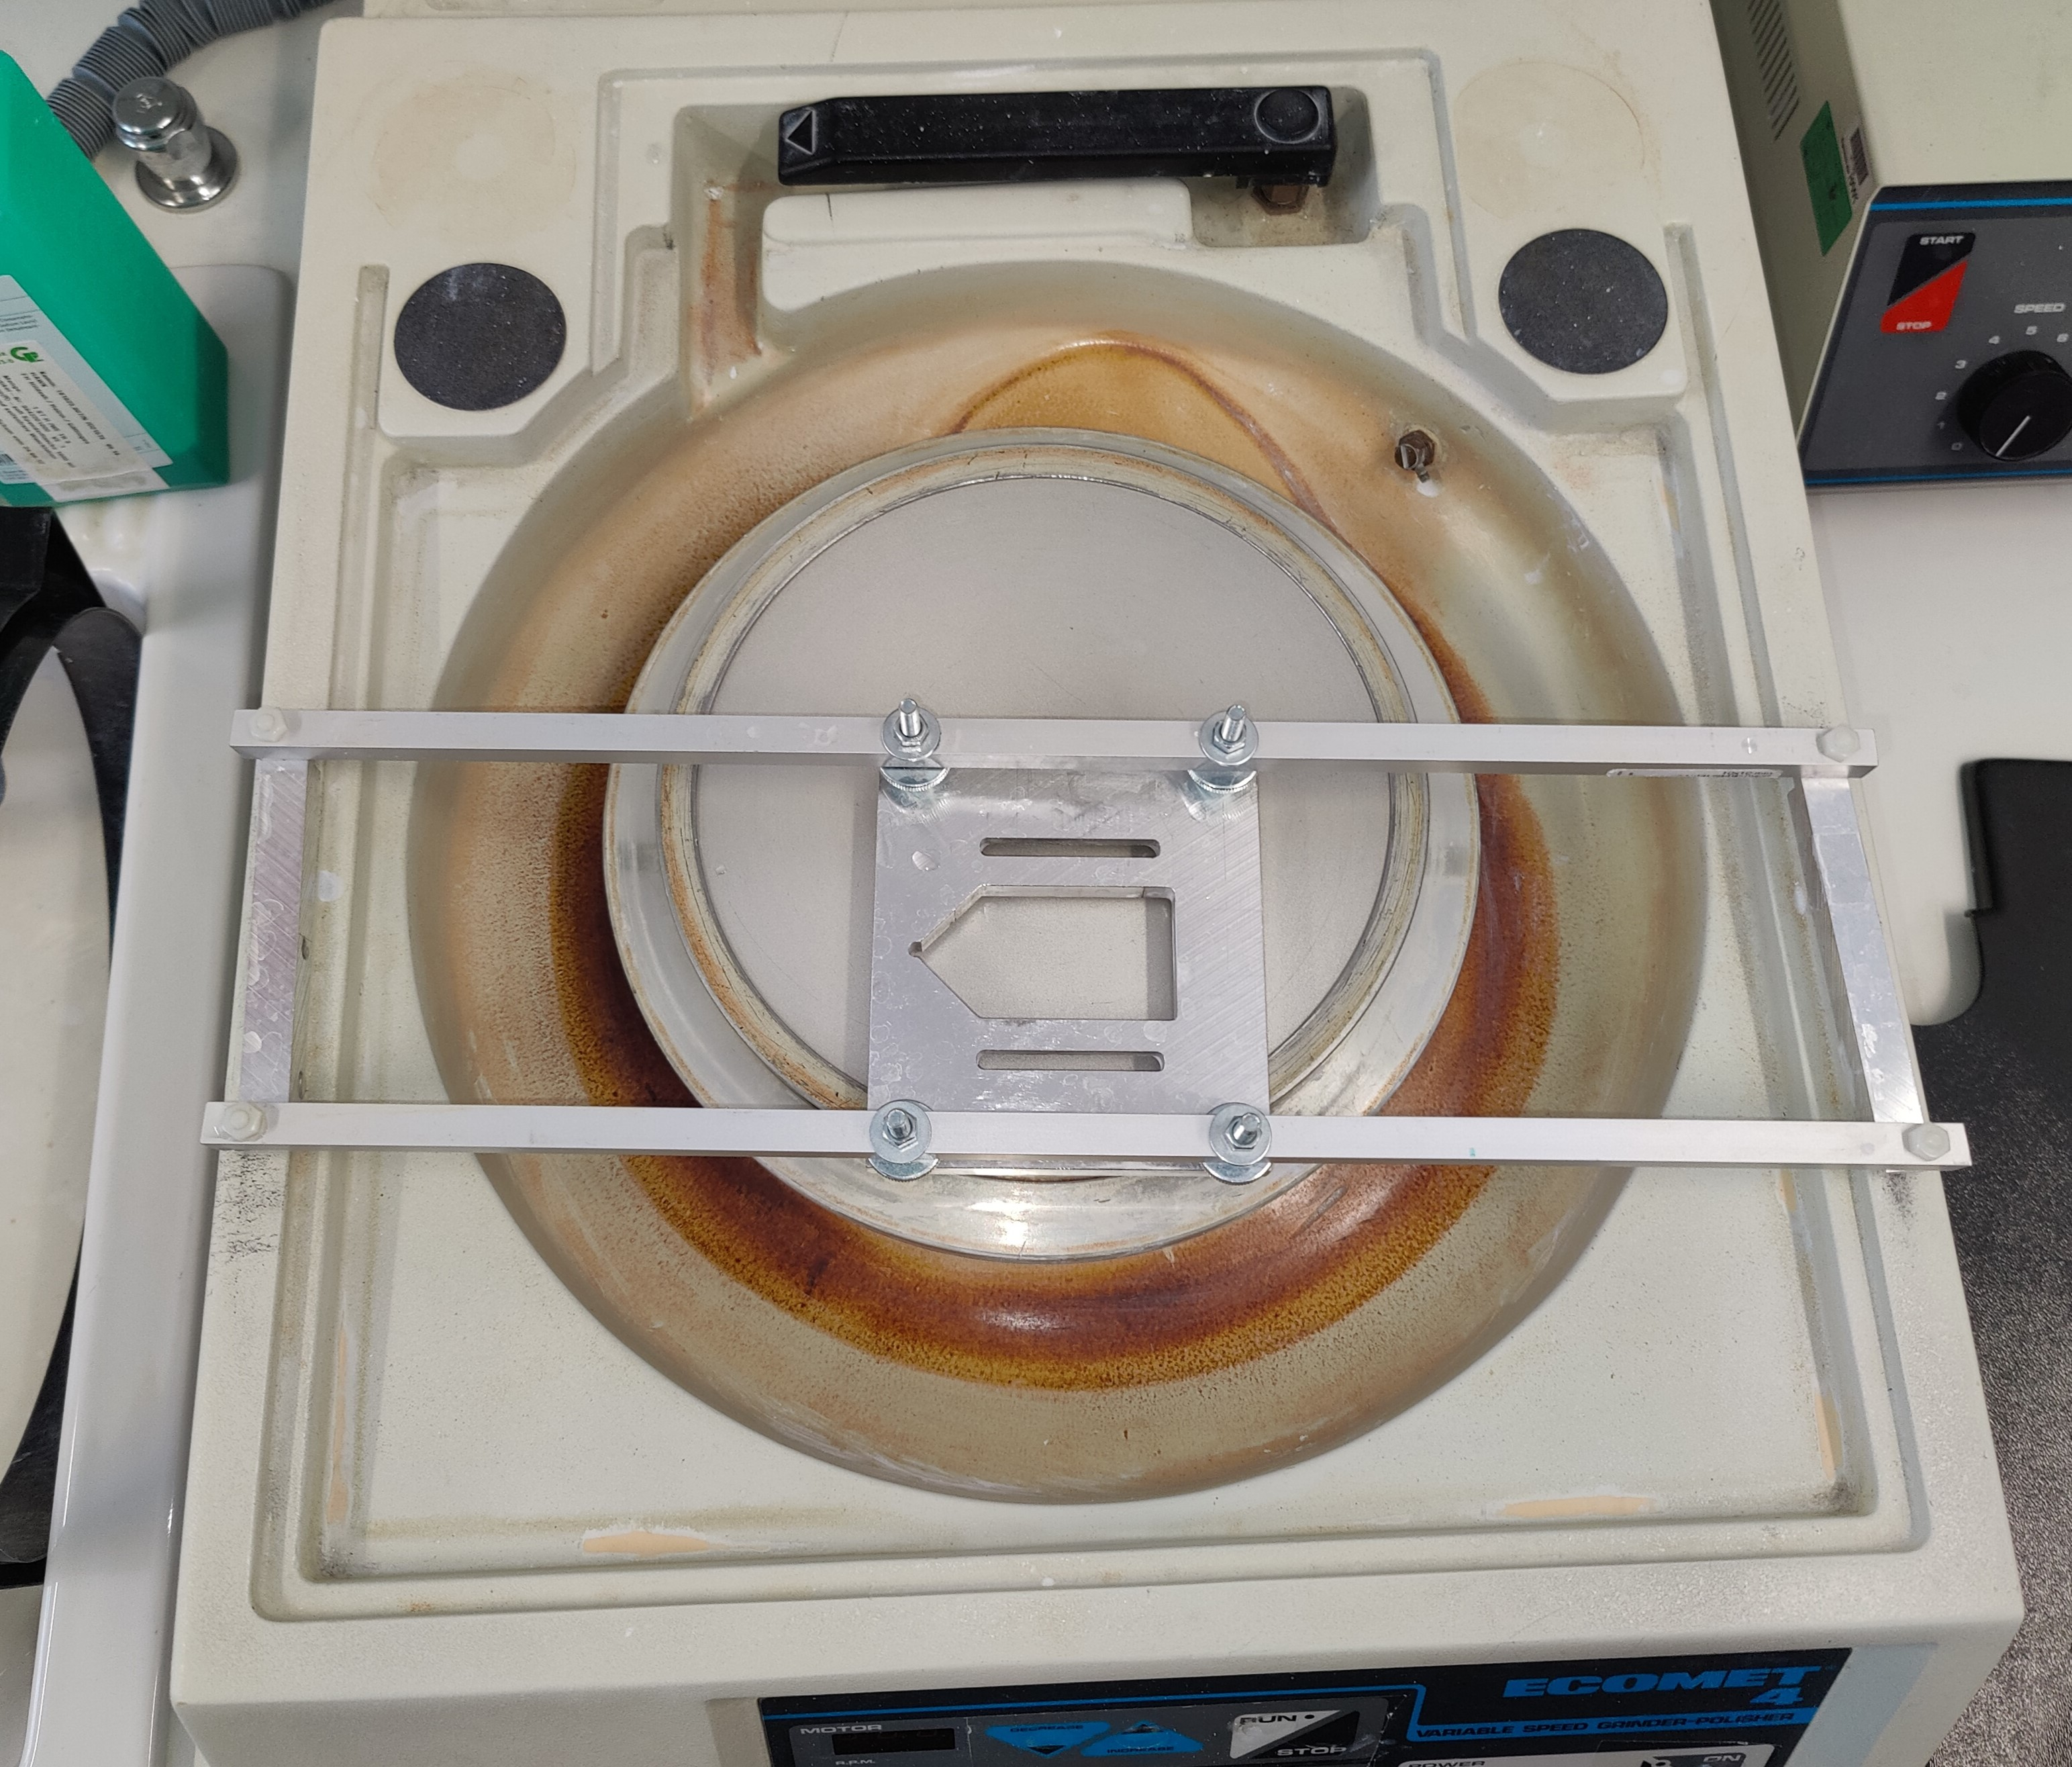
\includegraphics[width = 0.6\textwidth]{chapter_3/polish_setup_graphs/ecomet_holder.jpg} 
    %\vspace*{-30pt}
    \caption{Aluminum structure that constrained the movements of the holder.}
    \label{fig:aluminum_structure}
\end{figure}
In the end, the holder setup was completed utilizing a steel block with a weight of around $500\: g$, to create the necessary downforce with which to press the glass on the grinding or polishing surfaces. Considering that each of the glass sample had a diameter of $1\:cm$, the overall pressure felt by each piece is given by Equation~\ref{eq:pressure_on_glass}:
\begin{align}
    P=\frac{1}{2}\frac{gM}{\pi\left(d/2\right)^2}\approx30\ kPa \label{eq:pressure_on_glass}
\end{align}

\subsubsection{Grinding paper and polishing pad}
\label{subsubsec:grinding_paper_and_pad}
As for the grinding paper, a silicon carbide disk was employed, while for the polishing cloth, a magnetic backed 8 inches disk made of synthetic rayon was used.
\subsection{Parameters Chosen}
\label{subsec:parameters_chosen_polish}
To understand the relevant variables that could influence the introduction of contaminants in the glass, we had to choose a fixed number of possible parameters, from the ones listed at the start of Chapter~\ref{sec:pol_parameter}, that needed to vary between measurements.
\\
In a similar way done for the identification of the most valid LIBS parameter done in Chapter~\ref{subsec:parameters_chosen}, we did a set of tests to select the relevant variables that regarded the polishing process.

\subsubsection{Type of Glass}
Pure silica is not the only glass employed in optics, \ce{SiO2} is often doped with various compounds to tune the final refractive index of the material.
\\
The presence of other species could impact both physical and chemical properties of the glass, and, consequently, vary the contamination process.
\\
The two types of glass that were at our disposal were: pure silica, high purity samples provided by the manufacturer “QI Optiq”, and NZK-7, provided by the manufacturer “Schott”. 
\\
NZK-7 is a glass with a principal refractive index $n_d$, measured at $587.56 \: nm$, of 1.50847, and has an elemental composition displayed in Table~\ref{table:nzk7_concentration}:



\begin{table}[H]
    \centering
\begin{tabular}{|l|c|}
\hline
Chemical Name     & Concentration in Weight (\%) \\ \hline
Aluminum Oxide    & 1 - 10                         \\ \hline
Boron Oxide       & 10 - 20                        \\ \hline
Calcium Oxide     & \textless 1                  \\ \hline
Chlorine          & \textless 1                  \\ \hline
Sodium Oxide      & 1 - 10                       \\ \hline
Antimony Trioxide & \textless 1                  \\ \hline
Silica            & 60 - 70                        \\ \hline
Zinc Oxide        & 10 - 20                        \\ \hline
\end{tabular}
\caption{Chemical composistion of NZK-7 glass. }
    \label{table:nzk7_concentration}
\end{table}

In the composition it is important to notice the presence of compounds like aluminum oxide, calcium, zinc, and sodium. These elements are in fact part of the ones that we expect to introduce from the grinding and polishing process. Aluminum from the polishing suspension and the others from the tap water used in all the parts of the processing (the elemental composition of the tap water in Göttingen is shown in Table~\ref{table:water_composition}).
\\
The presence of these elements is confirmed by our measurements:
\begin{figure}[H]
    \centering
    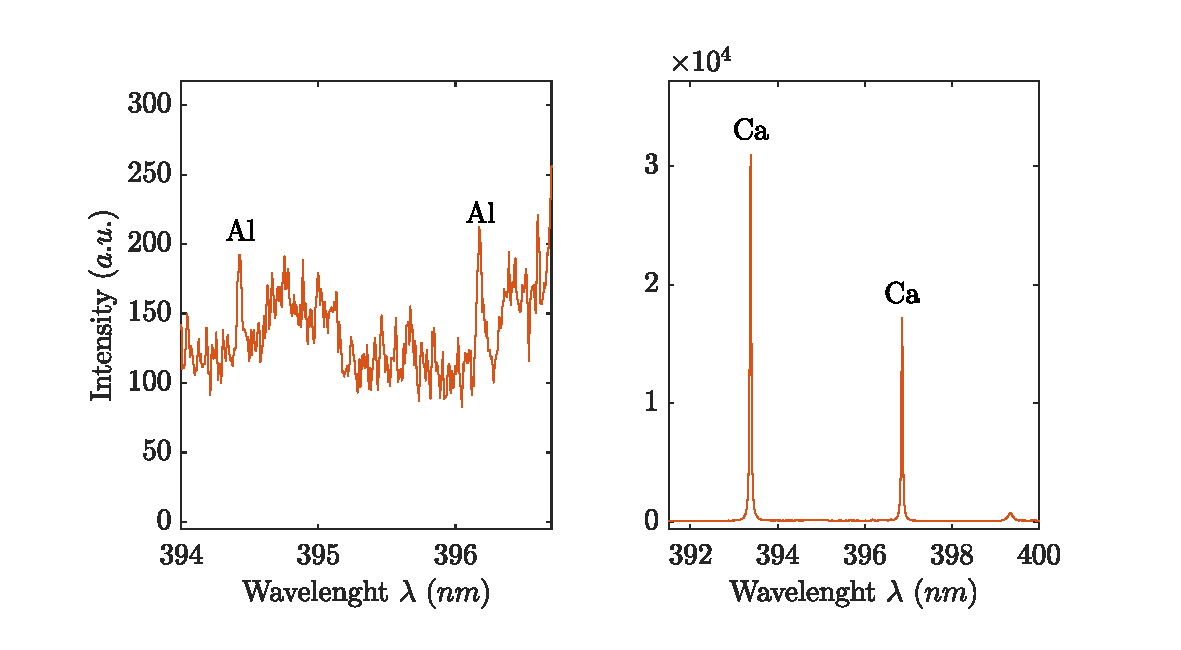
\includegraphics[width = \textwidth]{chapter_3/polish_setup_graphs/NZk7_contaminants_zoom.pdf} 
    \vspace*{-30pt}
    \caption{Focus on the aluminum and calcium peaks of NZK-7.}
    \label{fig:nzk7_aluminum_calcium}
\end{figure}
In Figure~\ref{fig:nzk7_aluminum_calcium} we can clearly see the presence of both aluminum and calcium peaks even in the “raw” sample. For this reason, we chose to not perform measurement on NZK-7 glass, it is much easier to track contaminants when the starting sample does not have the elements that we are searching for already in the spectrum.

\subsubsection{Type of Polishing Agent}
\label{subsubsec:polish_type_conc}
As already mentioned in Chapter~\ref{sec:pol_parameter}, the most common polishing suspensions used in optics manufacturing are \ce{Al2O3} and \ce{CeO2}. 
The specific products we employed were:

\begin{itemize}
    \item A cerium oxide-based mixture by the company GlassPolish, characterized by a particle size with an average of $2.5\: \mu m$ and a purity of more than 95\% as stated by the spec sheet.
    \item An aluminum oxide powder supplied by the company CharpauS, with a particle size between 2 and $6 \: \mu m$.
\end{itemize}

The limits of detection (LOD) of cerium and aluminum found in literature are, respectively, around $100 \: ppm$ and $1\: ppm$. [LOD taken from LIBS-info]
\\
By also looking at the theoretical emission spectra of cerium in Figure~\ref{fig:ce_plot_nist}, plotted from the information of the “relative intensity” on the NIST database, it is evident that there is no single peak that stands out and can therefore be easily identified. Emission lines cover almost continuously the whole spectrum from $350 \: nm$ to $500 \: nm$.
\begin{figure}[H]
    \centering
    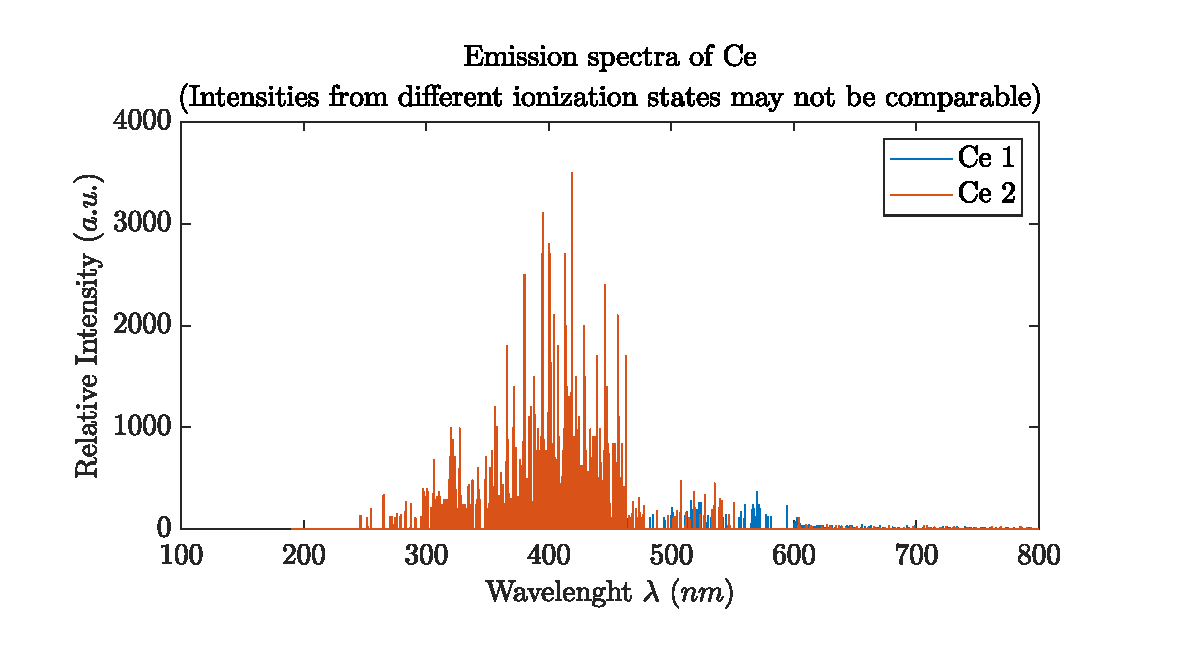
\includegraphics[width = \textwidth]{chapter_3/polish_setup_graphs/spectra_cerium.pdf} 
    \vspace*{-30pt}
    \caption{Spectra of cerium plotted from the information in the NIST database. }
    \label{fig:ce_plot_nist}
\end{figure}
This combined with the high LOD makes it particularly difficult to find this element in low concentrations using LIBS.
\\
In Figure~\ref{fig:ce_peaks_raw_polished} there is the comparison between the spectra of the same glass sample, raw and after one hour of polishing. In the highlighted spectral regions, there should be two intense cerium lines. It is clear that that even after 
\begin{figure}[H]
    \centering
    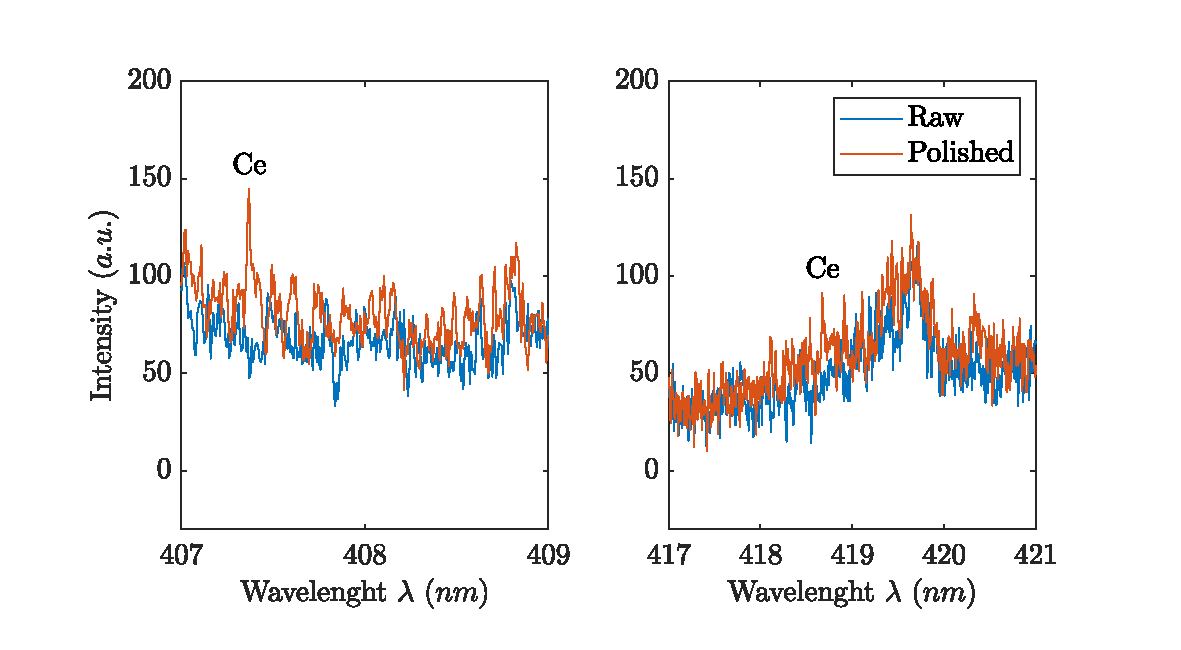
\includegraphics[width = \textwidth]{chapter_3/polish_setup_graphs/raw_polished_siO2_cerium.pdf} 
    \vspace*{-30pt}
    \caption{Cerium peaks compared in spectra before and after polishing. }
    \label{fig:ce_peaks_raw_polished}
\end{figure}
Under these conditions, it would be impossible to do any meaningful quantitative analysis. In the end we decided to focus our attention only on polishing with the alumina-based polishing agent.

\subsubsection{Polish Concentration}
\label{subsubsec:polish_concentration_setup}

As already mentioned in Chapter~\ref{sec:pol_parameter} the polish concentrations commonly used in optics manufacturing are between 5\% and 30\%. For our measurements we decided to take as sample concentrations 5\%, 15\% and 30\%. 

\subsubsection{Grinding and Polishing Times}
\label{subsubsec:grinding_pol_times}
Considering that diffusion is a time-dependent process we expect to have some dependencies on grinding and polishing time.
\\
To reduce the amount of variable we had to control, we decided to fix the grinding time to 3 minutes for every sample.
\\
Regarding polishing, expecting a dependence in the contaminants' concentration that was logarithmic/exponential with respect to time, we decided to take measurements not at fixed time intervals but instead to double the amount of time between each evaluation. From one minute to two hours of polishing.
\\
As a summary, the measurements were taken at: 
Raw, ground ($3\: min$), $1\: min$, $2\: min$, $4\: min$, $8\: min$, $15\: min$, $30\: min$, $1\: h$ and $2\: h$.

\subsection{Measurements of Polishing Components}
\label{subsec:measurements_pol_components}
In this section will be presented the results of LIBS analysis performed on all the components that were in direct contact with the samples and were therefore capable of introducing contaminants into the glass. In addition, a list of the elements dissolved in tap water is printed.

\subsubsection{Polishing Powders}
\label{subsubsec:meas_pol_powders}
LIBS analysis performed on a tablet of compressed aluminum oxide powder showed a very low presence of elements other than aluminum. Precisely calcium is present at a relative concentration lower than 1\% while only a few traces of copper and gallium were detected.

\subsubsection{Silicon Carbide Grinding Paper}
\label{subsubsec:grinding_paper_meas}
Some LIBS analyses were also performed on a sample of unused grinding paper. Sodium was found to be present at a very high relative concentration of about 10\%. A small portion of contaminants such as calcium and iron were found with concentrations lower than 0.5\%, while the presence of other traces elements, such as magnesium and lanthanum, was also detected with concentrations in the order of few ppm.

\subsubsection{Polishing Pad}
\label{subsubsec:polishing_pad_meas}
The polishing pad was also subjected to the same kind of analysis. Not surprisingly, the results of the measurement showed that the main component of the pad is carbon, as it is the main constituent of the rayon fiber. Silicon has also been found present with a relative concentration of about 5\% while calcium only in concentrations smaller than 1\%.


\subsubsection{Tap Water Chemical Composition}
\label{subsubsec:polishing_pad_meas}
The type of water mostly used in the optics manufacturing industry is tap water. In Germany, public water quality is periodically checked and an elemental composition analysis for the tap water in Göttingen is easily accessible from public databases. In Table~\ref{table:water_composition} are shown the main elements dissolved in the water we used during both the grinding and polishing processes:

\begin{table}[H]
    \centering 
    \begin{tabular}{|l|c|c|}
    \hline
                                   & Unit   & \multicolumn{1}{l|}{Value Range} \\ \hline
    Water Temperature              & °C     & 5,9-16,7                                  \\ \hline
    PH Value                       &        & 7,7-8,2                                   \\ \hline
    Total alkaline earths          & mol/m³ & 1,4                                       \\ \hline
    Calcium                        & mg/l   & 40,1-42,5                                 \\ \hline
    Magnesium                      & mg/l   & 7,33-9,03                                 \\ \hline
    Sodium                         & mg/l   & 7,4-10,9                                  \\ \hline
    Potassium                      & mg/l   & 0,9-1,3                                   \\ \hline
    Chloride                       & mg/l   & 10,8-14,7                                 \\ \hline
    Nitrate                        & mg/l   & 14,9-19,3                                 \\ \hline
    Sulfate                        & mg/l   & 25-35                                     \\ \hline
    Phosphorus Compounds           & mg/l   & \textless{}0,1                            \\ \hline
    Silicon Compounds              & mg/l   & 5,0-7,4                                   \\ \hline
    Organically Bound Carbon (TOC) & mg/l   & 0,7-1,0                                   \\ \hline
    Aluminum                       & mg/l   & 0,02-0,03                                 \\ \hline
    Oxygen                         & mg/l   & 9,2-13,0                                  \\ \hline
    \end{tabular}
    \caption{Chemical composition of tap water in Göttingen in 2023.}
        \label{table:water_composition}
    \end{table}

With the goal of partially mitigating the contamination process on the surface of the glass sample caused by water, some experiments were carried out employing only distilled water from the start to the end of the procedure.
\\
This was particularly challenging due to the need to ensure the contact of the glass only with instruments washed with distilled water, from the glassware, where the polishing slurry was prepared, to the tweezers used to handle the samples. The grinding paper and the polishing pad also had to be replaced constantly for the same reason.
\\
But due to the extremely high solubility of distilled water, the risk of accidentally dissolving species into the solution was always a concern.

\section{Other apparatuses}
\label{sec:other_apparatuses}
Other than LIBS, experiments were also carried out on FTIR, XPS and contact angle measuring systems. Since they were not the focus of our research, in this section will be presented only a brief description of the apparatuses we used.

\subsection{FTIR}
\label{subsec:ftir_setup}
For FTIR measurements we employed the “Frontier” apparatus manufactured by PerkinElmer.
\\
Considering that our main concern regarded finding contaminants at the surface of our samples, we used a setup to perform “Internal Reflectance Spectroscopy”, a technique we described in short in Chapter~\ref{sec:ftir}.
\\
During measurements, a lot of issues were caused by the lack of consistency between different evaluations of the same sample measured multiple times in a row, in the same exact conditions. A crucial requirement of this technique is achieving perfect contact between the glass and the high refractive index material in the machine, using a plastic spacer to ensure even pressure on the small glass sample was not enough.
\\
Even though the presence and position of the absorption peaks remained constant, the absolute value of the absorption could vary a lot.
\\
In Figure~\ref{fig:ftir_issues} are shown different FTIR measurements of the same sample, the runs were done by simply removing and replacing the material from the apparatus.

\begin{figure}[H]
    \centering
    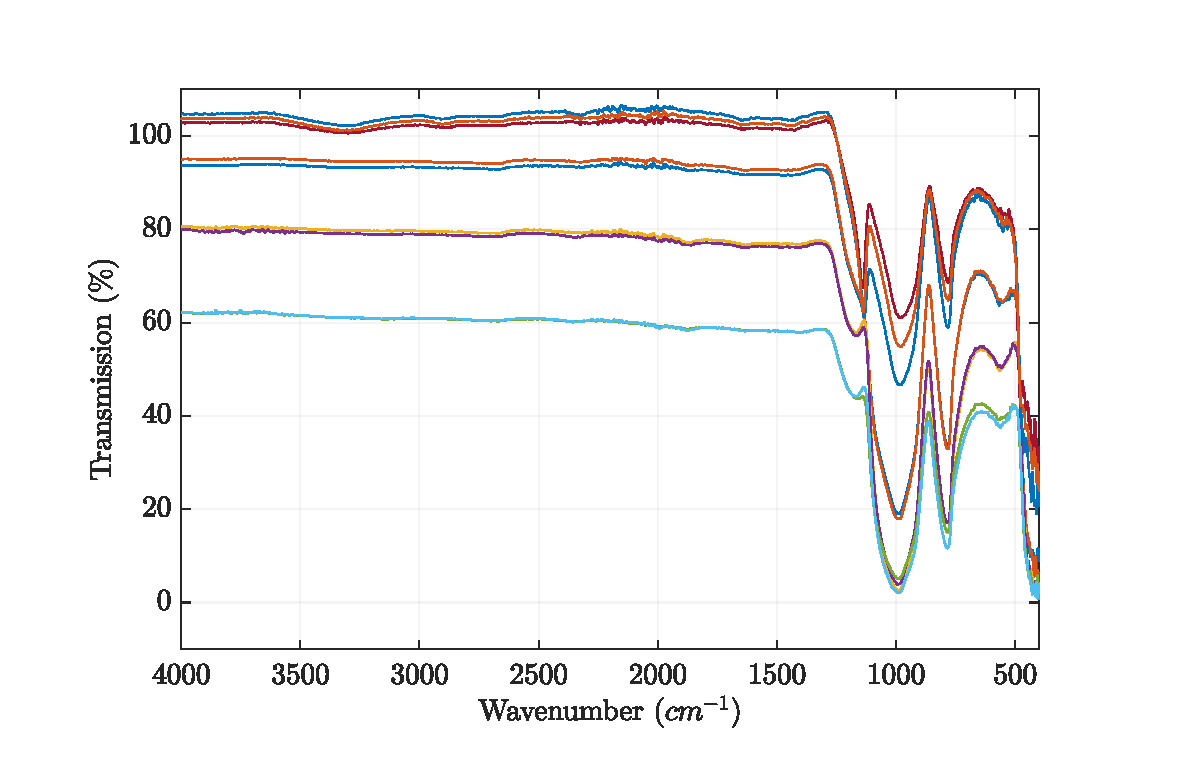
\includegraphics[width = \textwidth]{chapter_3/other_apapratuses_graphs/FTIR_issues.pdf} 
    \vspace*{-30pt}
    \caption{Various FTIR measurements made to the same sample with internal reflectance spectroscopy.}
    \label{fig:ftir_issues}
\end{figure}

In the plot we can see that even the transmission at the wavenumber range between 4000 and $1500\: cm^{-1}$, that for glass should always be around 100\%, spans from more than 100\% to 60\%.

\subsection{Contact Angle Measurement}
\label{subsec:contact_angle_setup}
The contact angle measurement apparatus was provided by the Kruss company, specifically, the DSA100E automated system.
\\
Experiments were carried out using water (\ce{H2O}) and diiodomethane (\ce{ CH2I2}) as, respectively, polar and apolar probe liquids.
\\
This technique is very sensible to surface characteristics and particular attention must be paid to avoid unwanted depositions of external substances. In our case, we discovered that cleaning between measurements with isopropanol could heavily influence the evaluation of the contact angle.  
\\ 
By looking at the surface of the glass with a microscope, as shown in Figure~\ref{fig:surface_droplets}, we could clearly see the presence of microdroplets of isopropyl alcohol, even hours after the cleaning. 

\begin{figure}[H]
    \centering
    \includegraphics[width = 0.8\textwidth]{chapter_3/other_apapratuses_graphs/surface_droplets.png} 
    %\vspace*{-30pt}
    \caption{Surface of a glass sample cleaned with isopropanol.}
    \label{fig:surface_droplets}
\end{figure}

To ensure that the droplets were evaporated completely, the samples were put in an oven for 40 minutes at a temperature of $60\: ^{\circ} C$ after each cleaning.

\subsection{XPS}
\label{subsec:xps_setup}
The XPS apparatus that measured our samples is a PHI VersaProbe II from Ulvac-phi. The model uses a monochromatic \ce{Al-K$\alpha$} source with a photon energy of $1486.6 \: eV$. The applied X-ray source has a power of 100 W.
\\
As explained in Chapter~\ref{sec:xps}, the XPS analysis is sensitive to just a few monolayers of the surface of the sample. To carry out depth resolved examinations, a small portion of the sample is removed from the surface with ion etching and consecutive measurements are conducted until the desired depth is reached.
\\
In our case, z-resolution was not one of the focuses of our research, so the XPS measurements were done only one time per sample, after surface cleaning had been performed with ion etching.

